\documentclass[12pt]{article}
    \usepackage[final]{pdfpages}
    \usepackage{listings} %For code in appendix
    \usepackage{hyperref}
    \usepackage{alltt}
    \usepackage{color}
    \usepackage{sectsty}
    \usepackage{layout}
    
    \definecolor{dkgreen}{rgb}{0,0.6,0}
    \definecolor{gray}{rgb}{0.5,0.5,0.5}
    \definecolor{mauve}{rgb}{0.58,0,0.82}
    \chapterfont{\color{blue}}
    \sectionfont{\color{cyan}}
    \font\myfont=cmr12 at 40pt
    \lstset
    {
        frame=tb,
        language=C++,
        aboveskip=3mm,
        belowskip=3mm,
        showstringspaces=false,
        columns=flexible,
        basicstyle={\small\ttfamily},
        numbers=none,
        numberstyle=\tiny\color{gray},
        keywordstyle=\color{blue},
        commentstyle=\color{dkgreen},
        stringstyle=\color{mauve},
        breaklines=true,
        breakatwhitespace=true
        tabsize=1
    }
    \setlength{\topmargin}{-13pt}

    \title{\myfont Lab 3}
    \date {\myfont 3rd week}
    \author{\myfont FIT Staff}
    \begin{document}
    \maketitle

    \section{Topics}
        \begin{itemize}
            \item\large Arrays
            \item Loop operators: for, while, do while
        \end{itemize}

    \section{Reading Materials}
        \large In Russian
        \begin{itemize}
            \item \small \url{https://informatics.msk.ru/mod/book/view.php?id=559}
            \item \small \url{https://informatics.msk.ru/mod/book/view.php?id=559&chapterid=297}
        \end{itemize}
        In English
        \begin{itemize}
            \item \small \url{http://www.cplusplus.com/doc/tutorial/arrays/}
        \end{itemize}

        \section{Problem Set}
        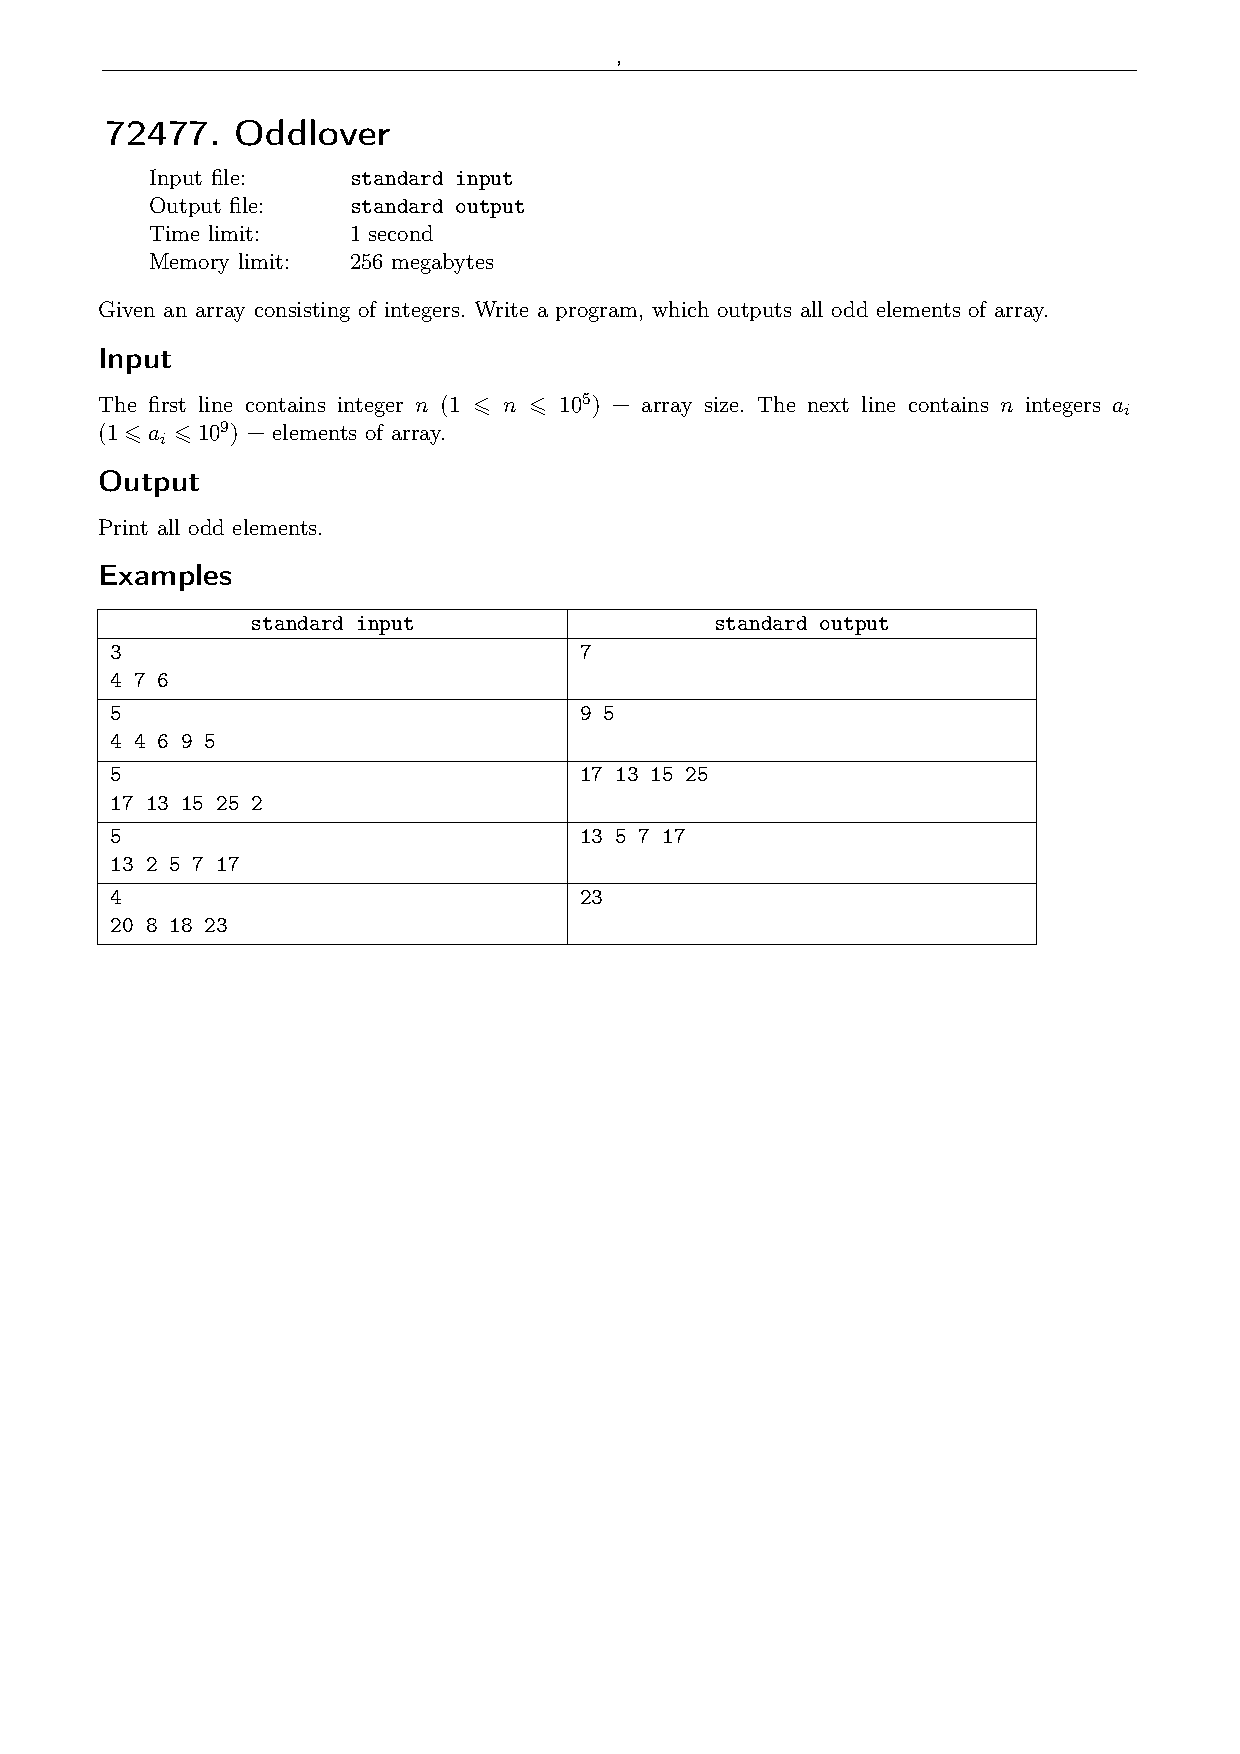
\includepdf[pages=-]{72477.pdf}
        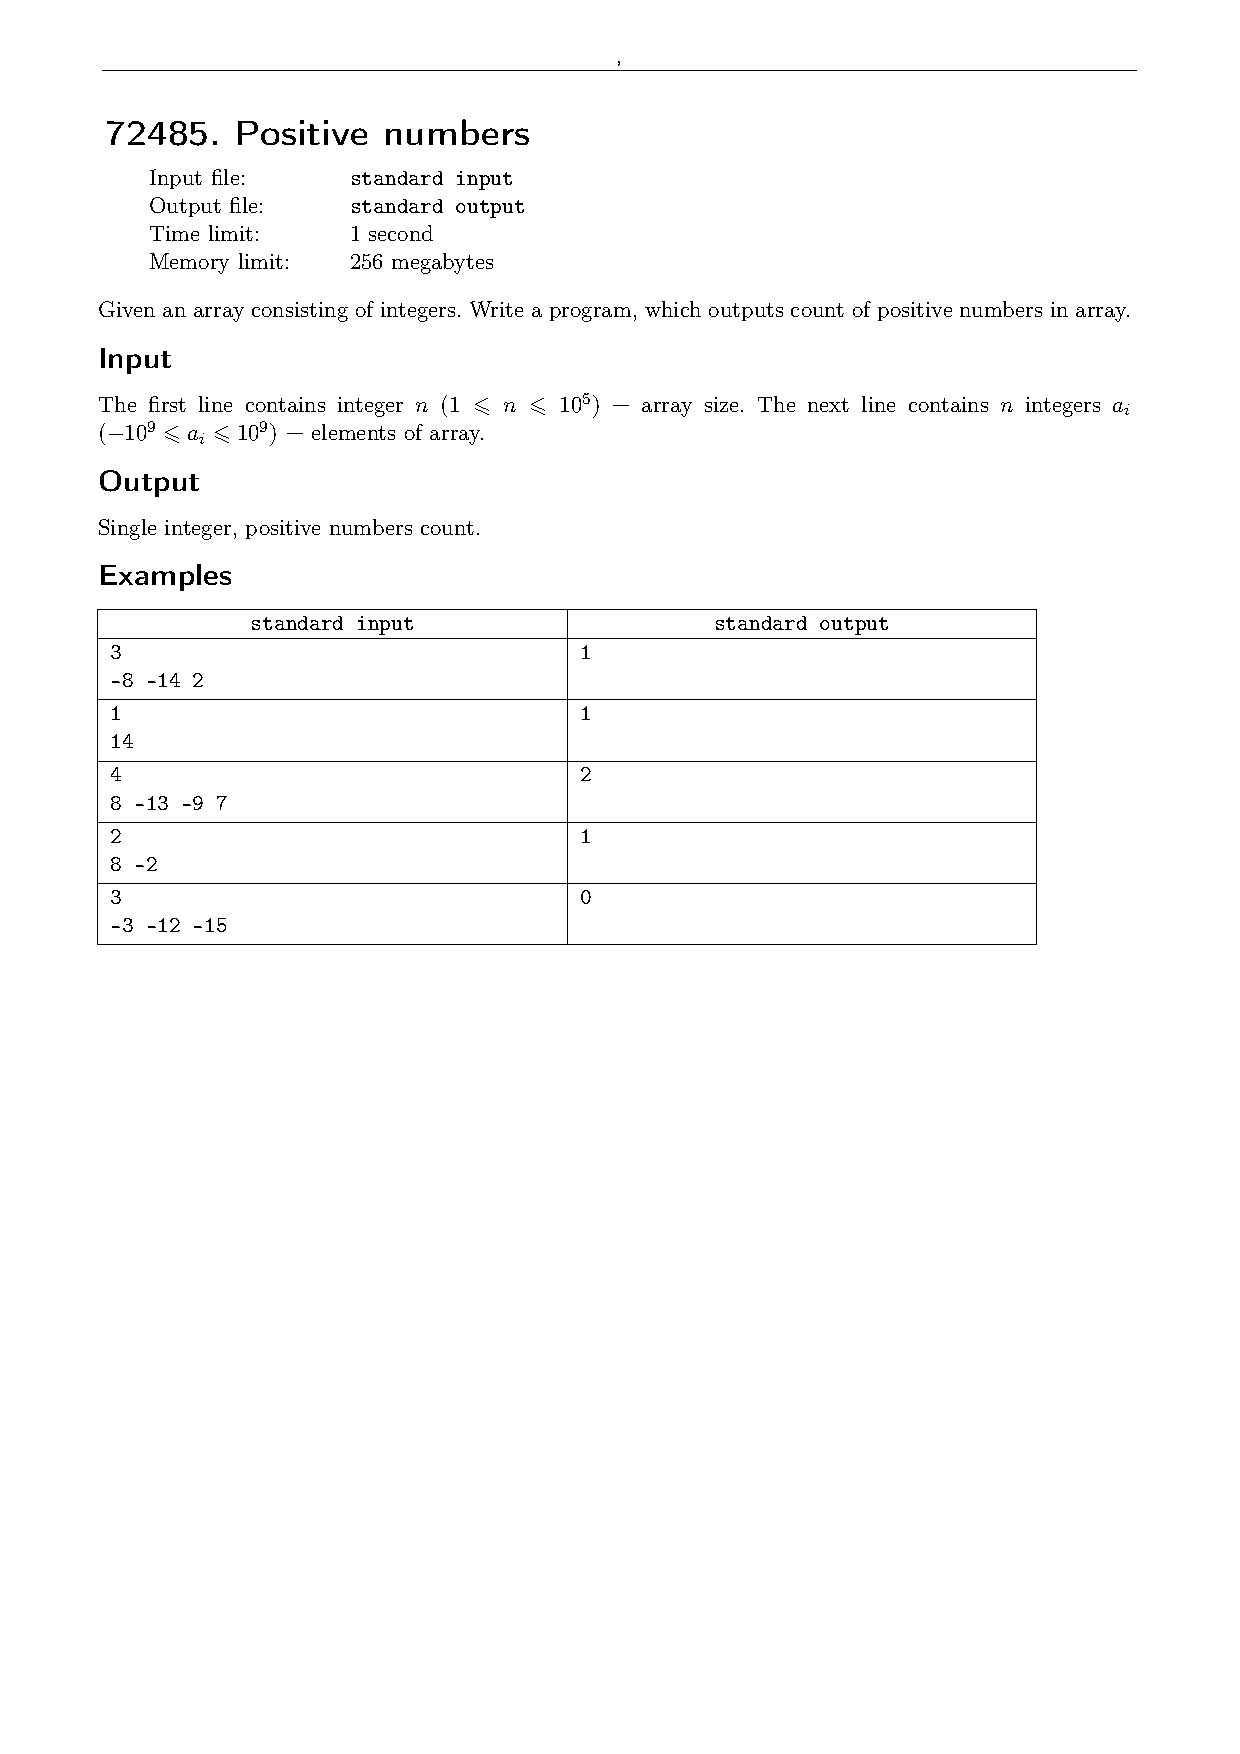
\includepdf[pages=-]{72485.pdf}
        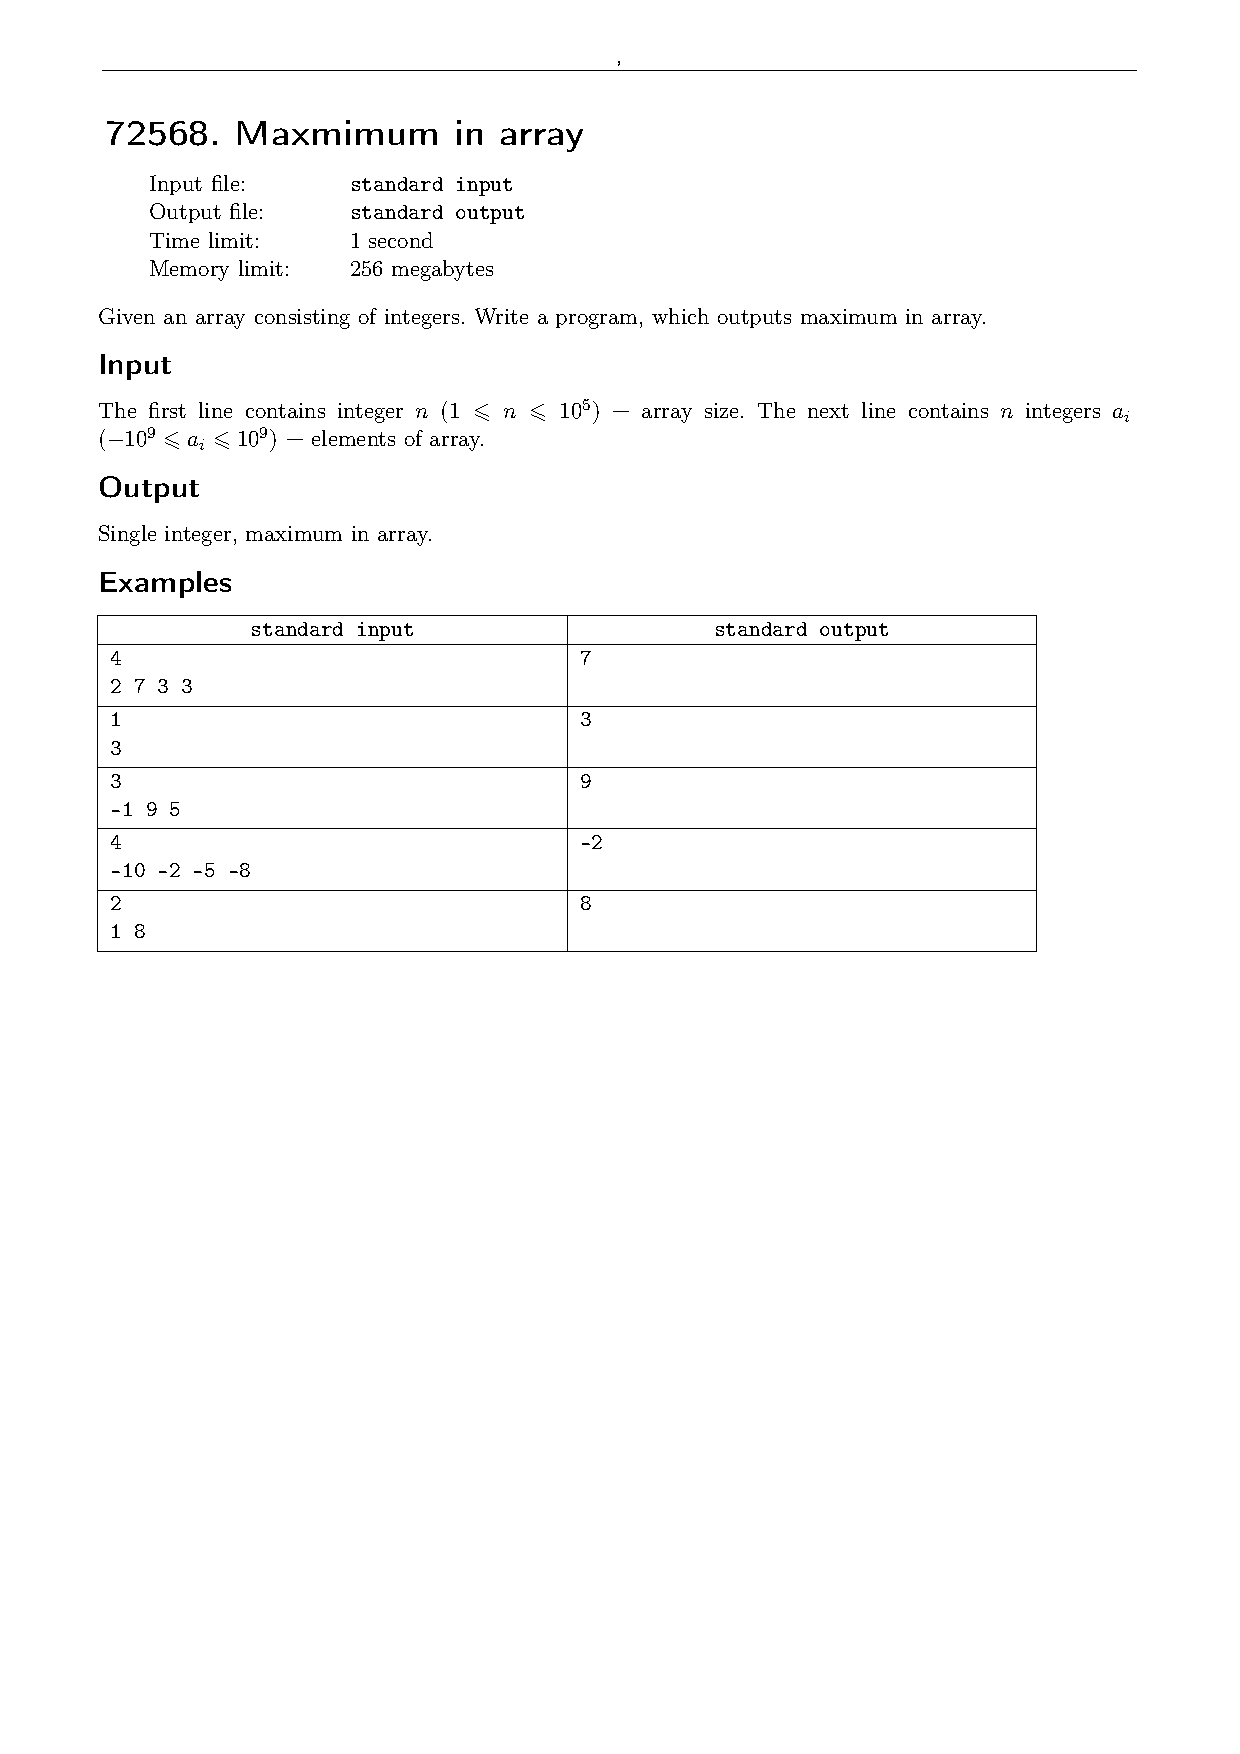
\includepdf[pages=-]{72568.pdf}
        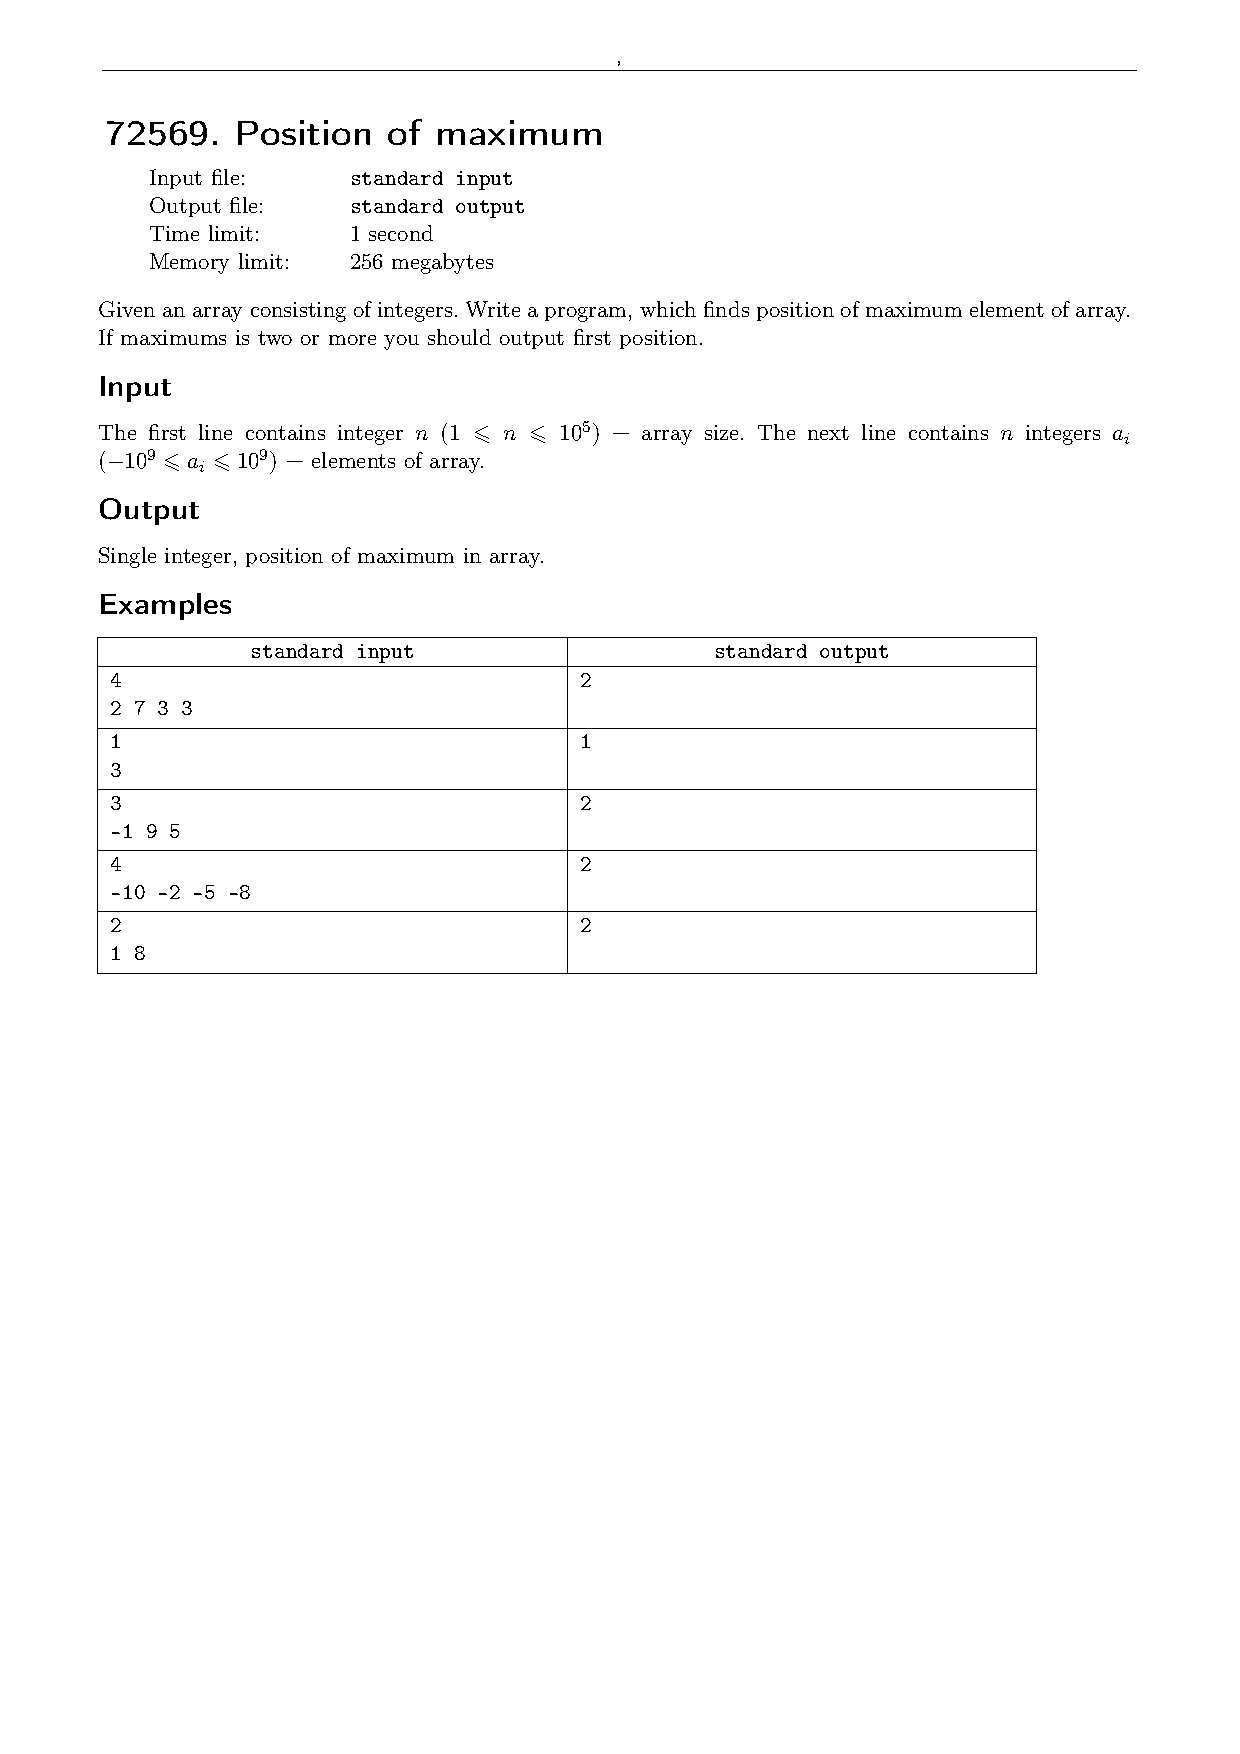
\includepdf[pages=-]{72569.pdf}
        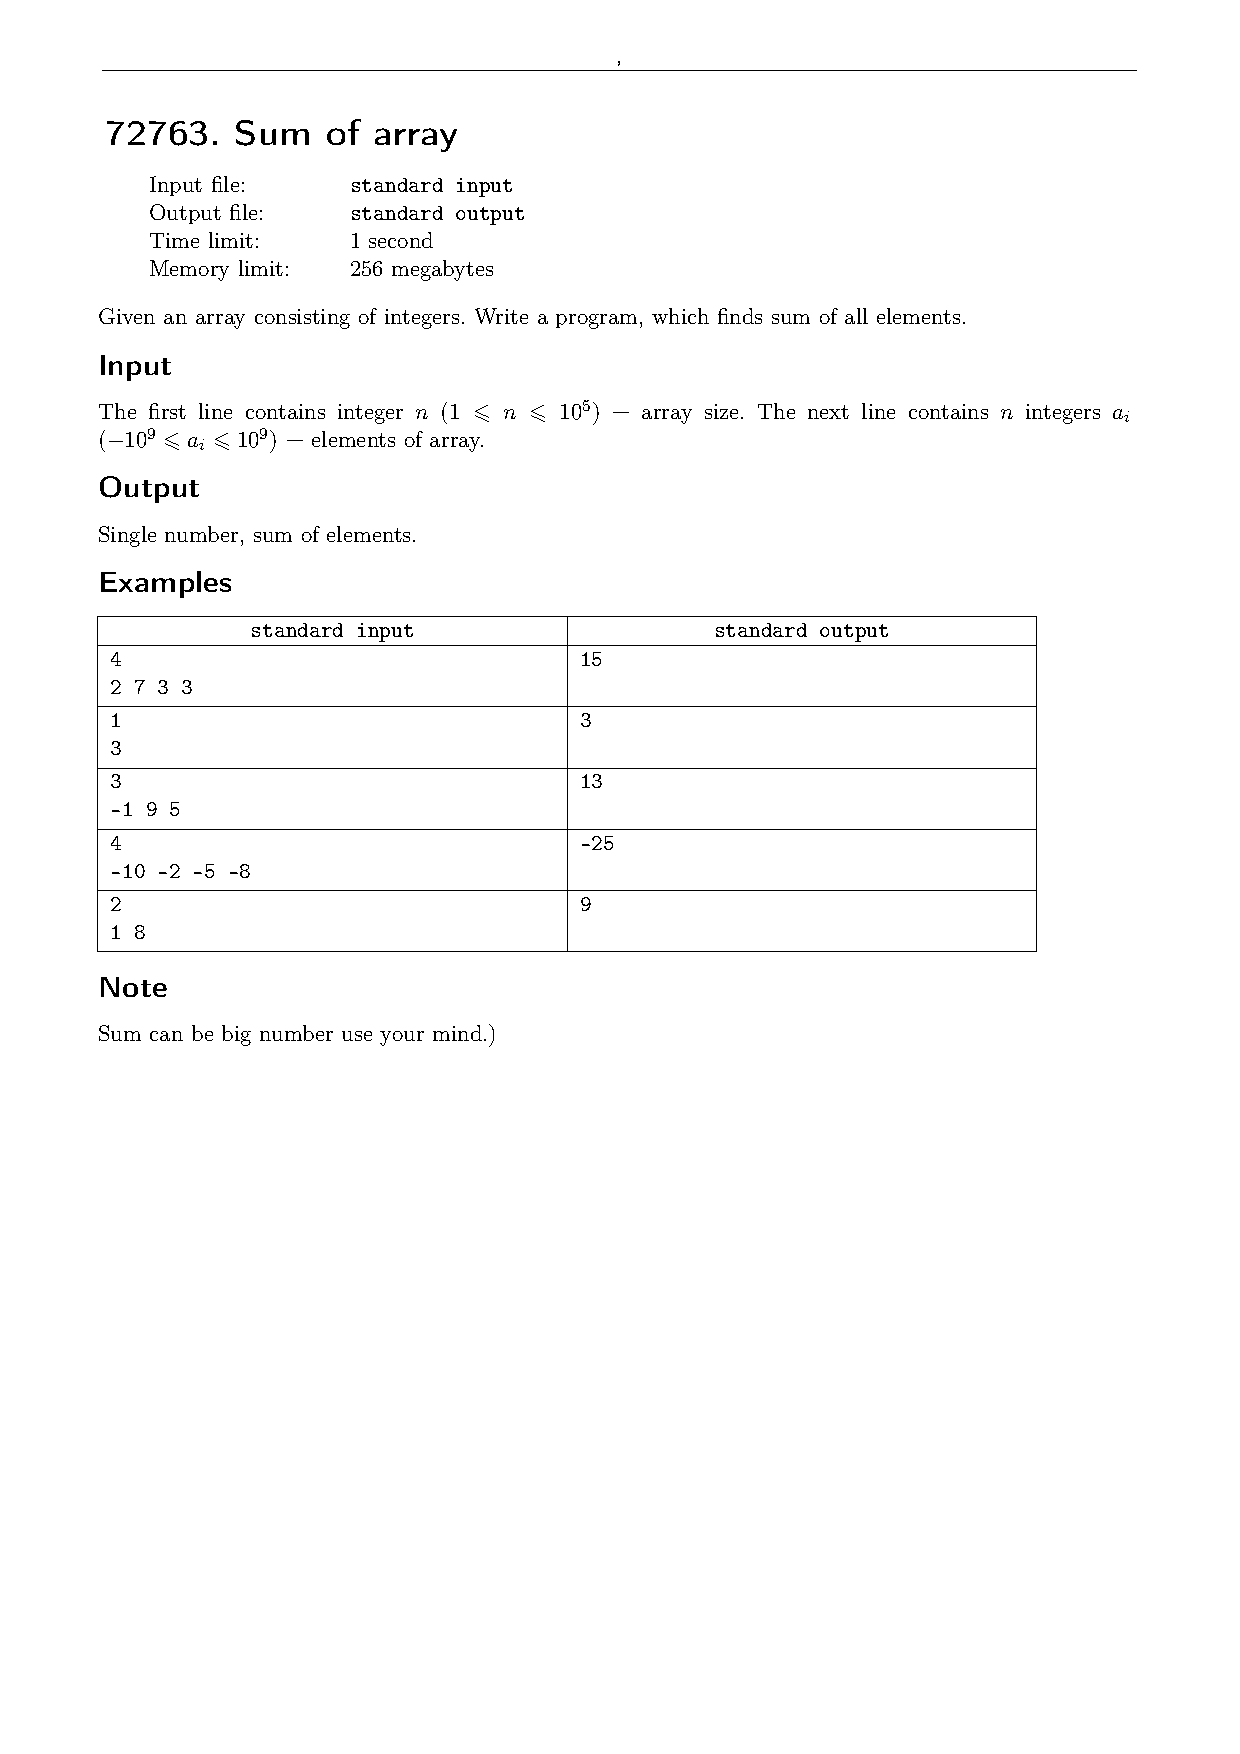
\includepdf[pages=-]{72763.pdf}
        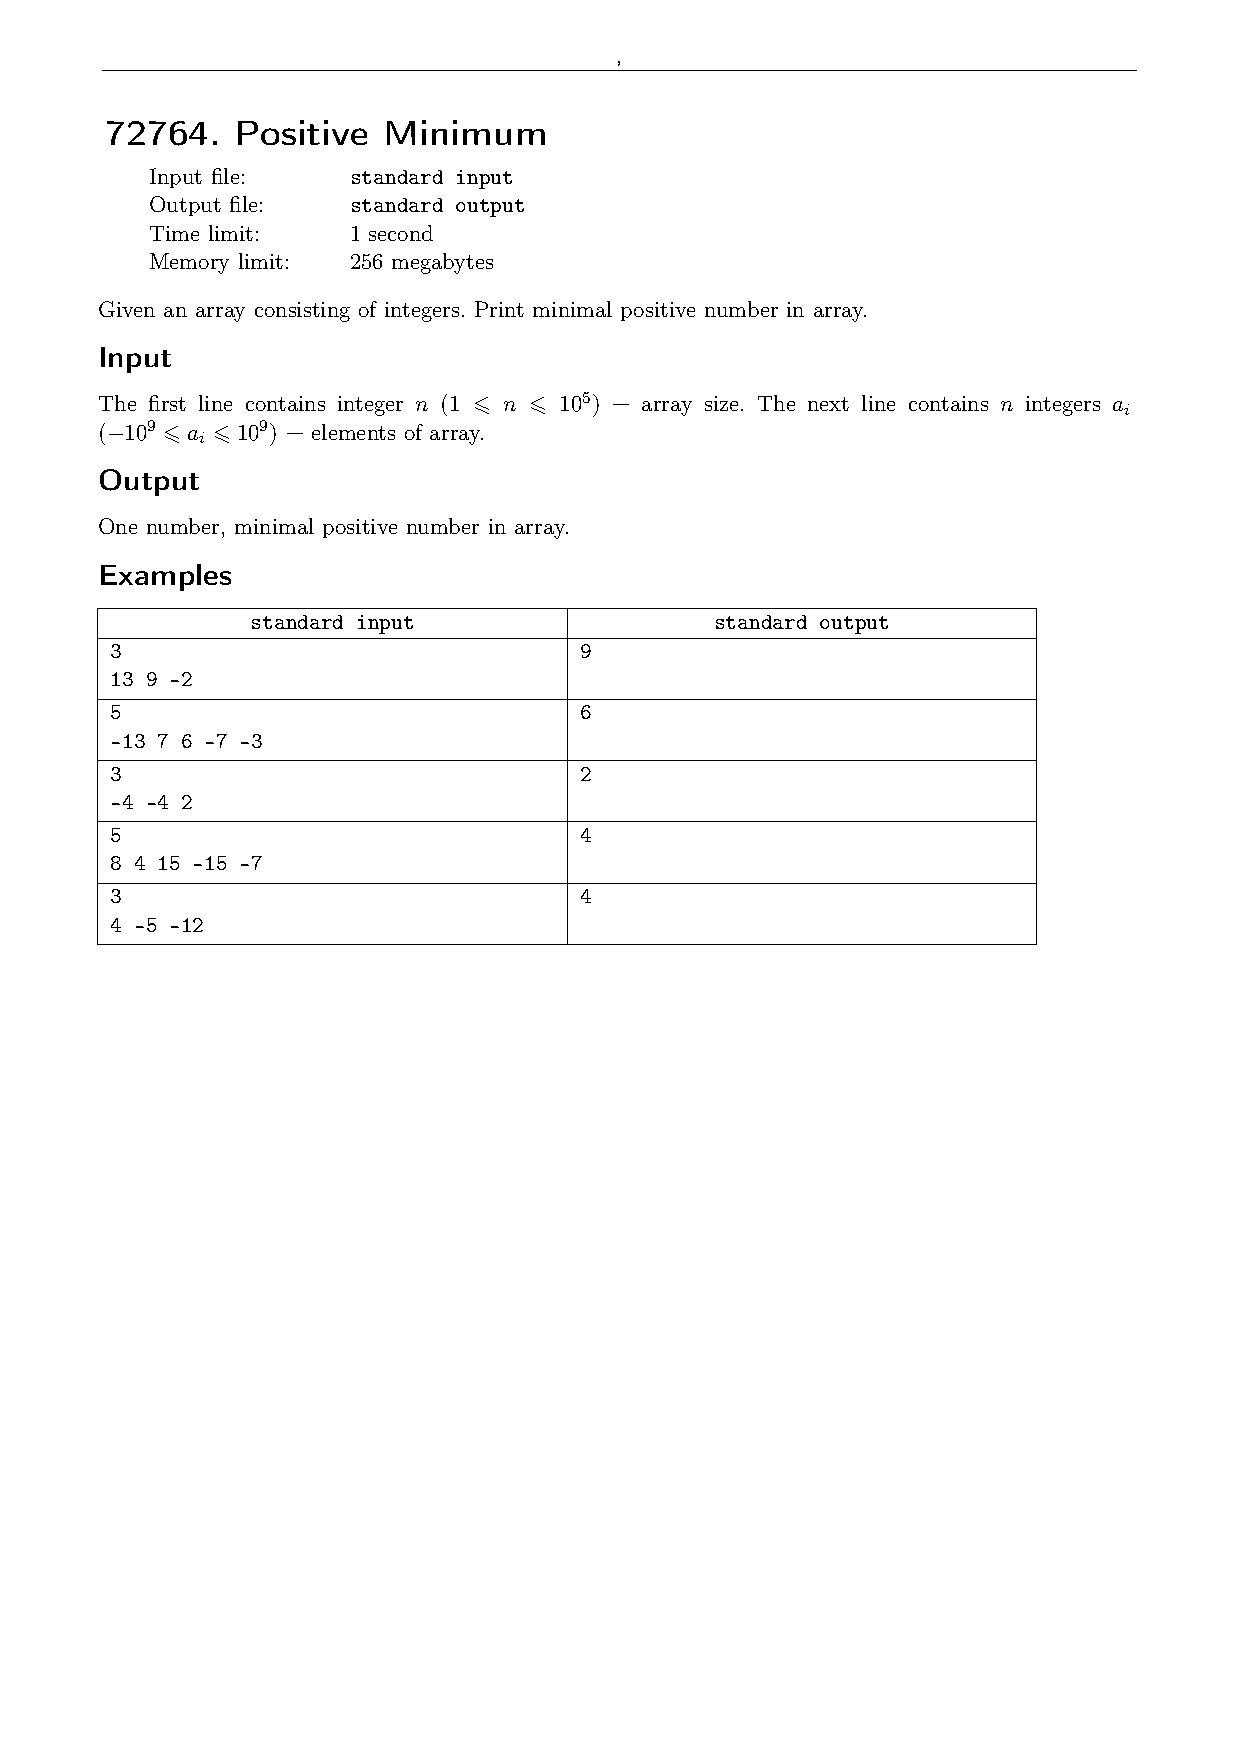
\includepdf[pages=-]{72764.pdf}
        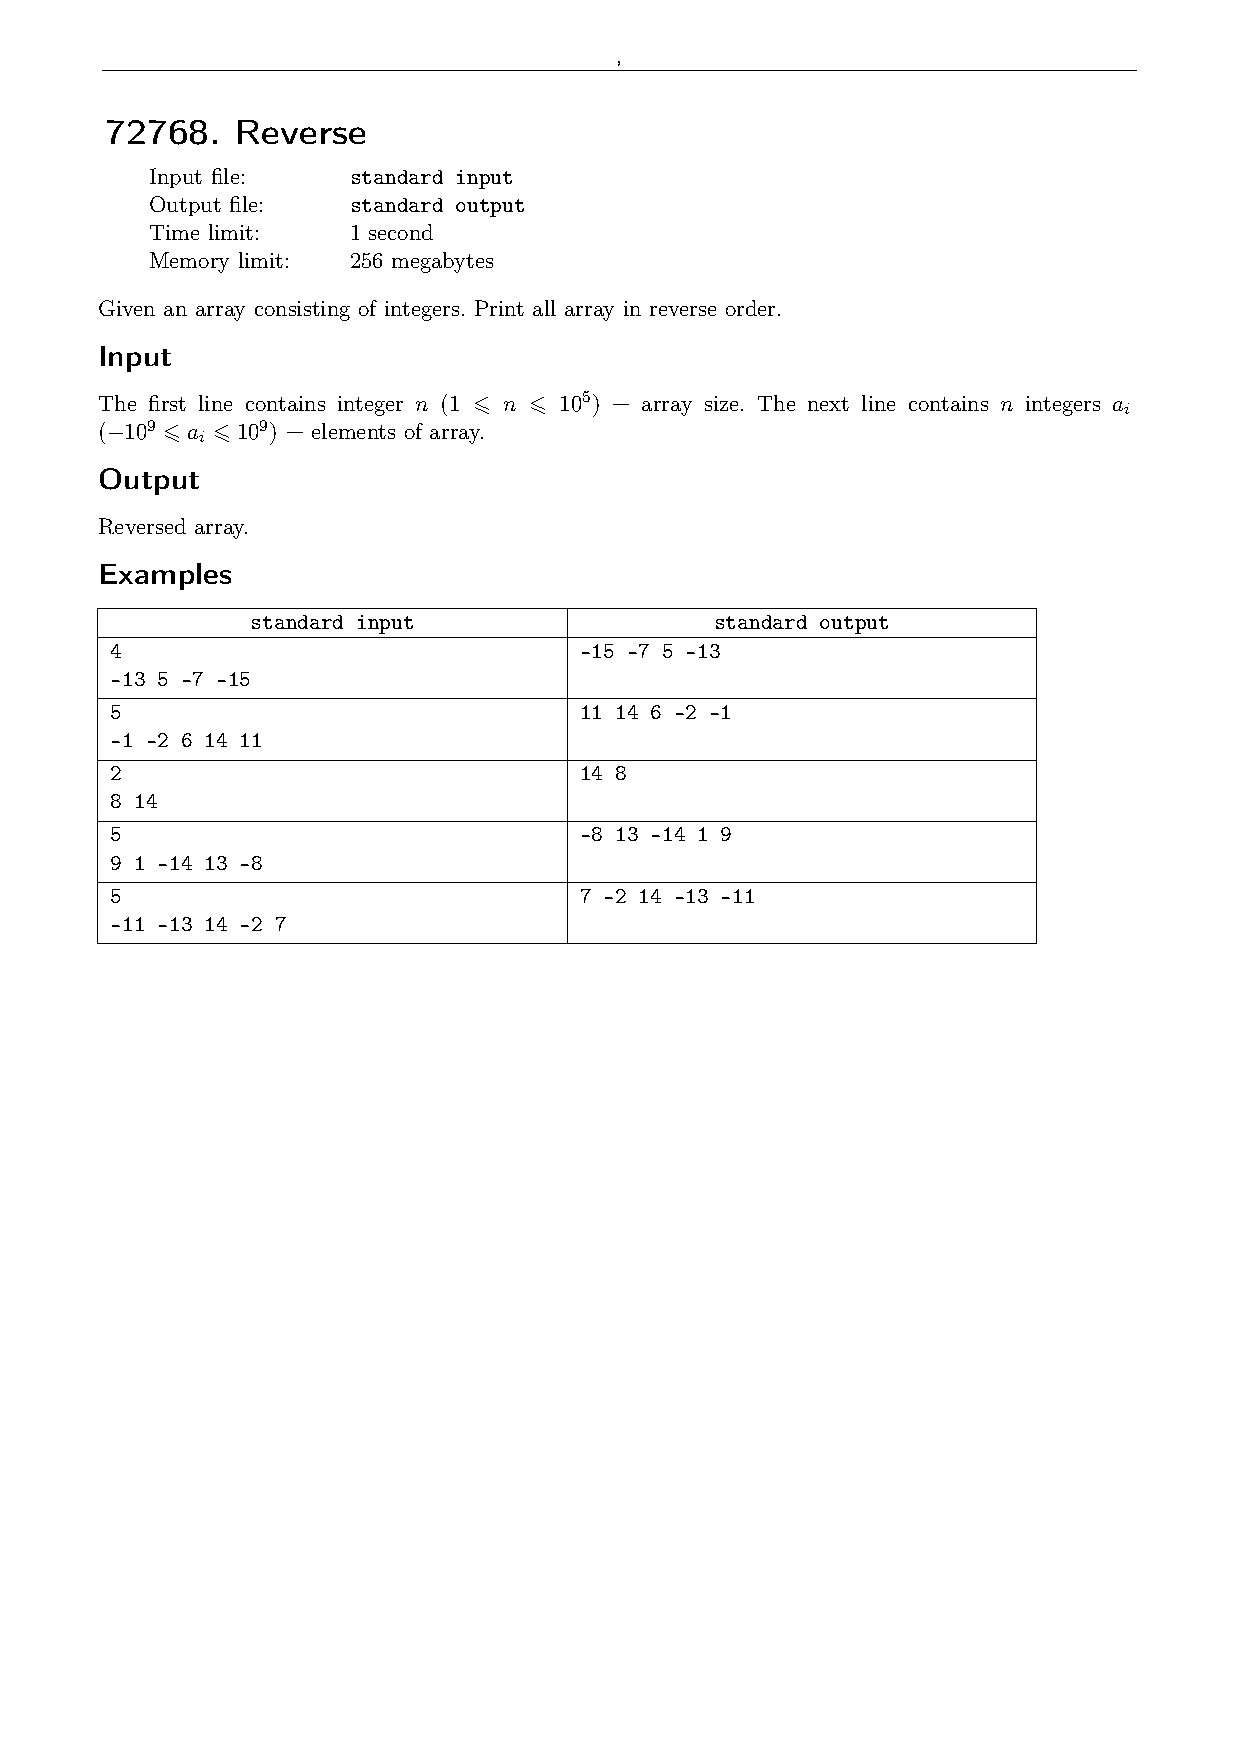
\includepdf[pages=-]{72768.pdf}
        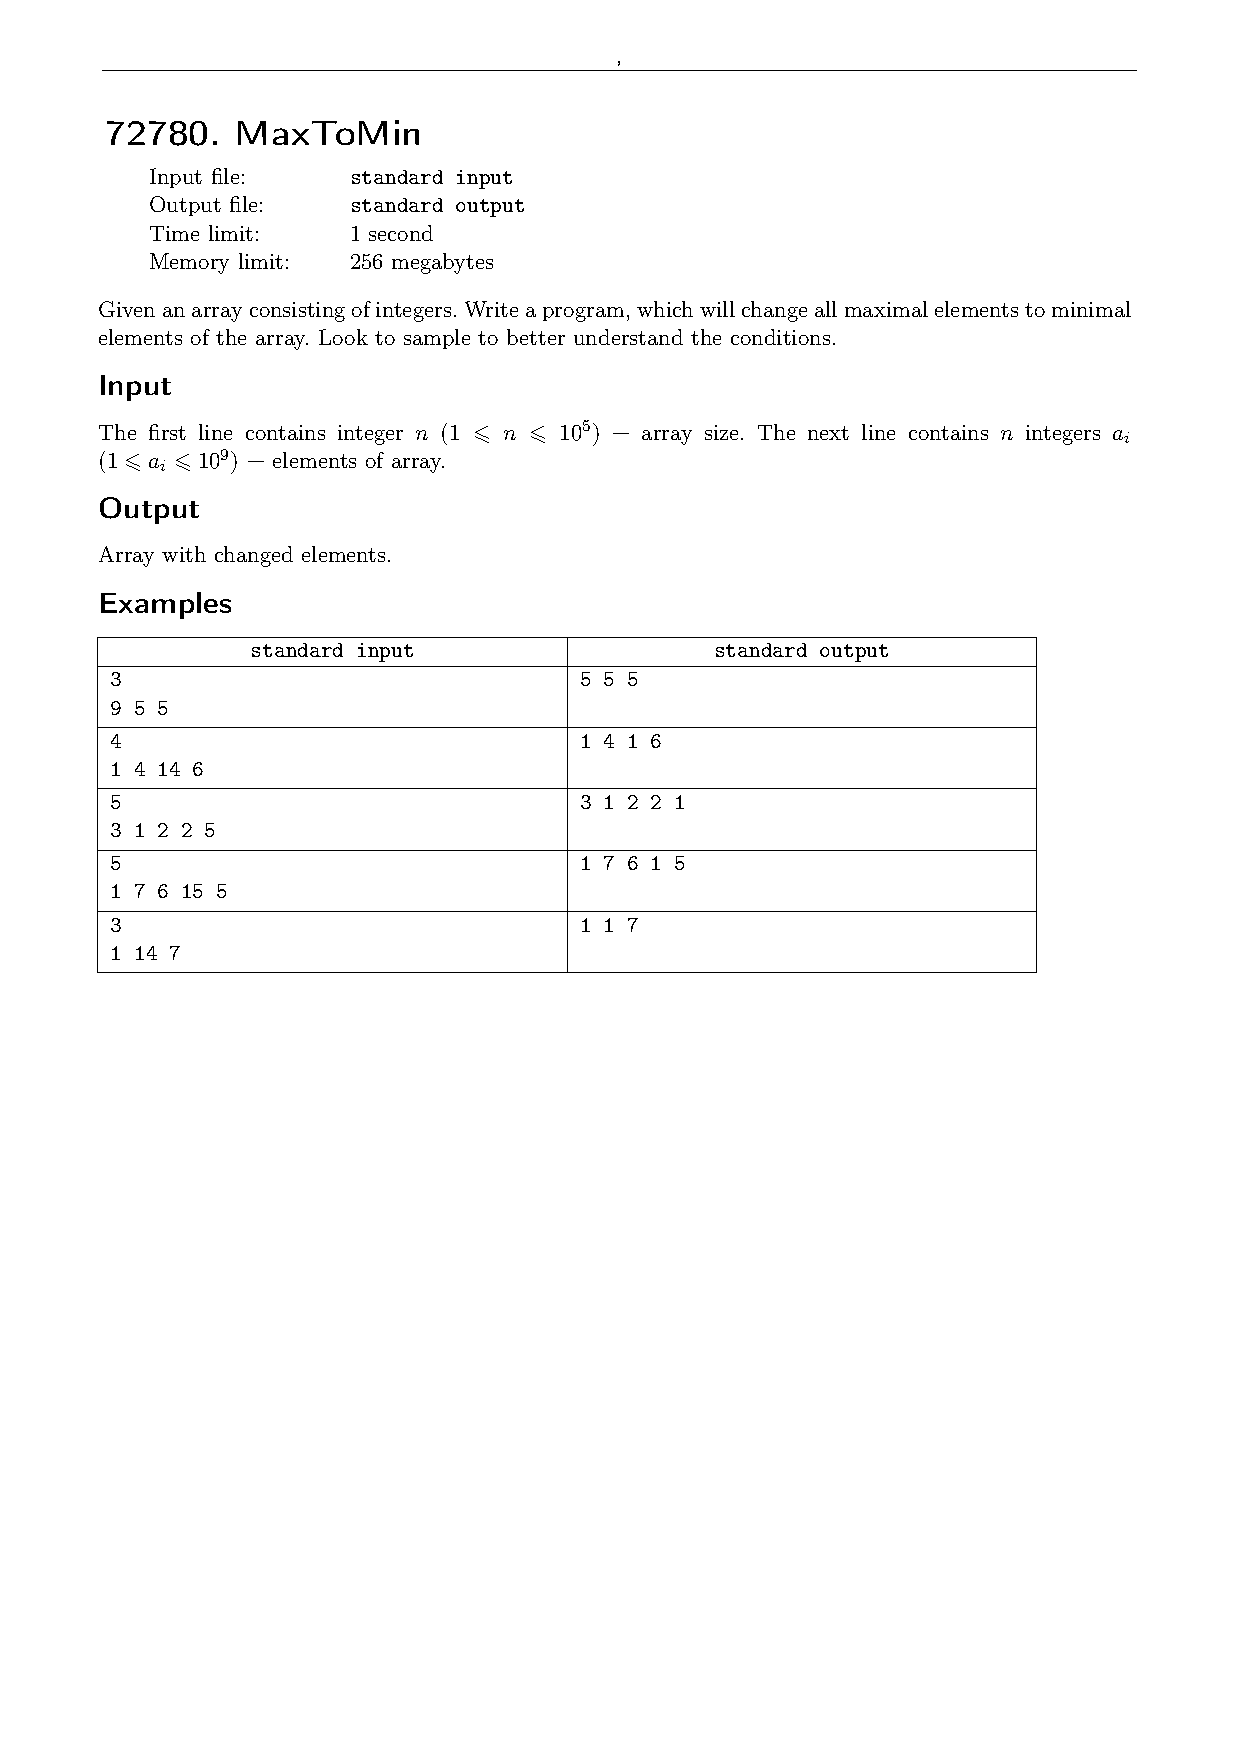
\includepdf[pages=-]{72780.pdf}
        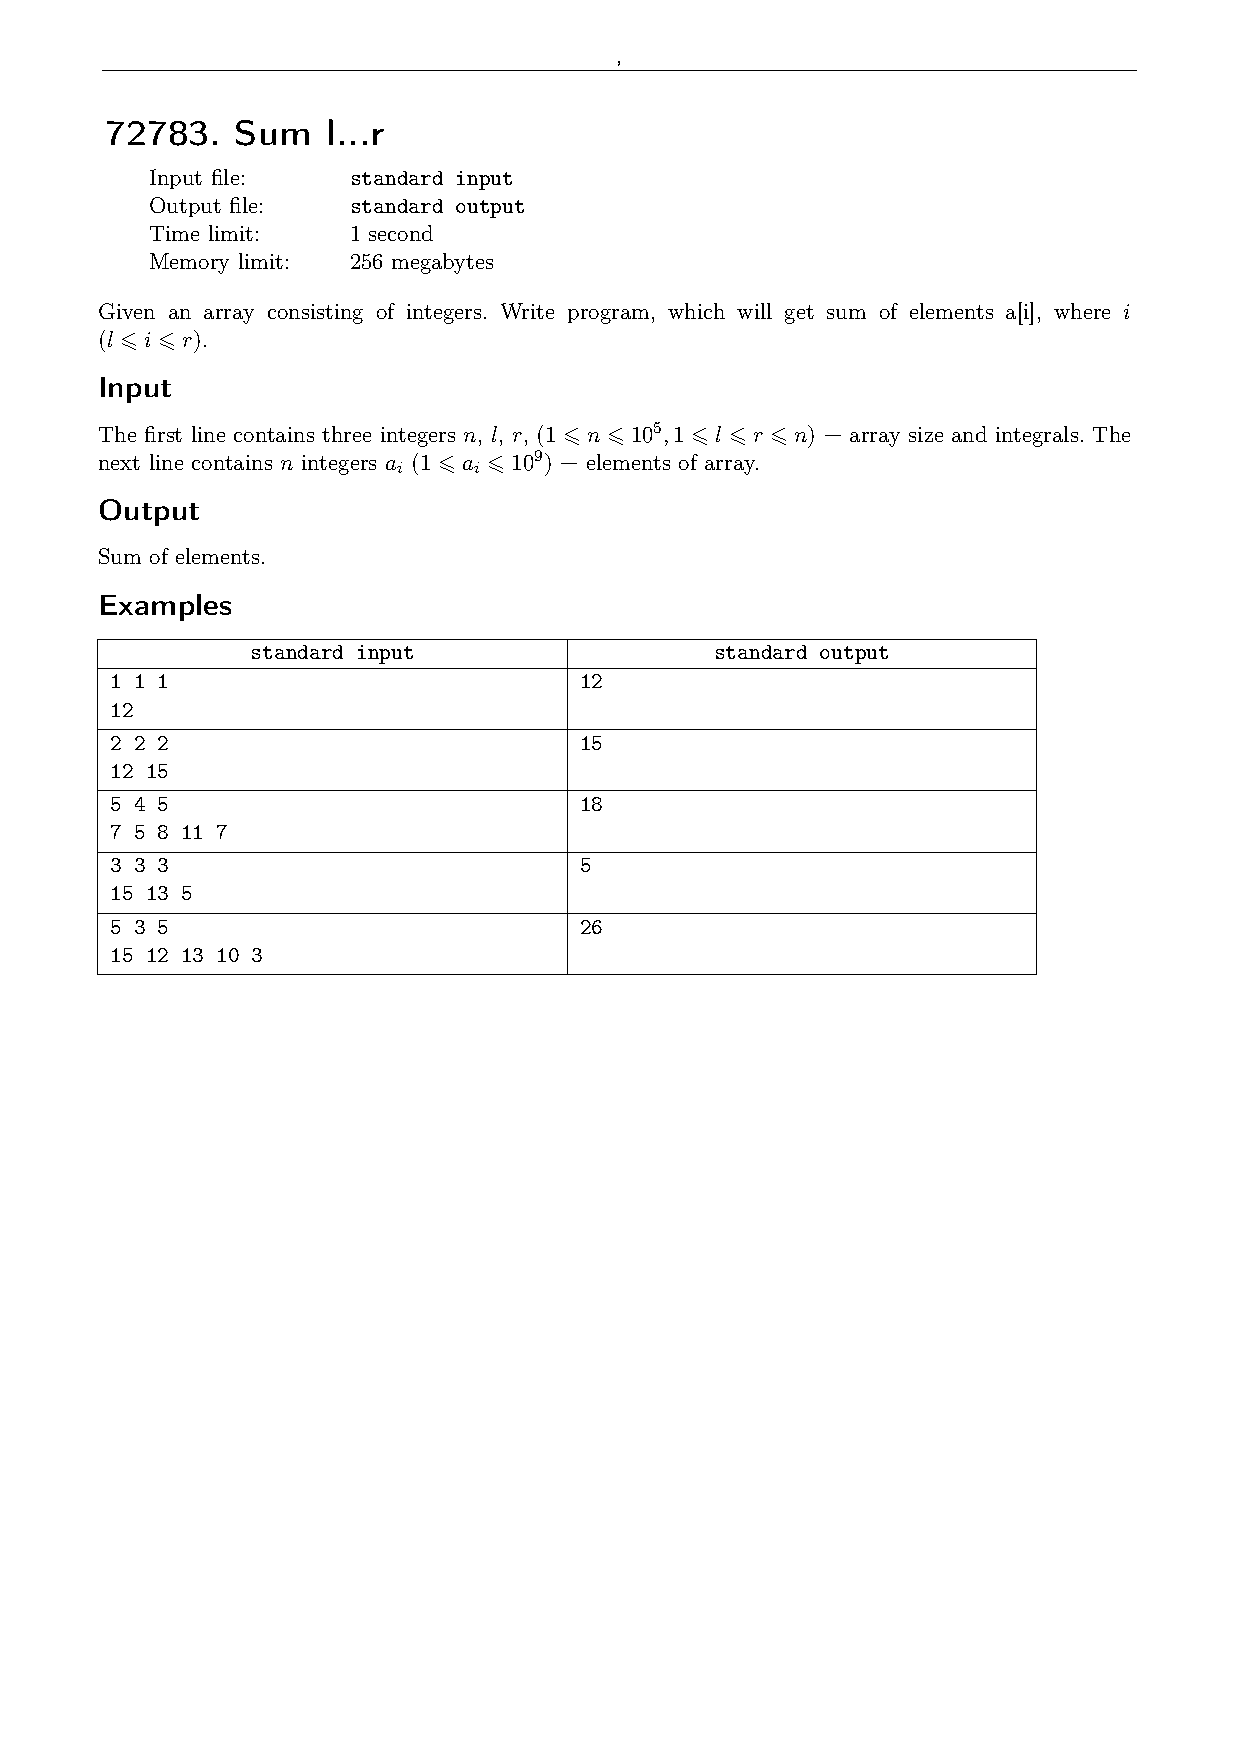
\includepdf[pages=-]{72783.pdf}
        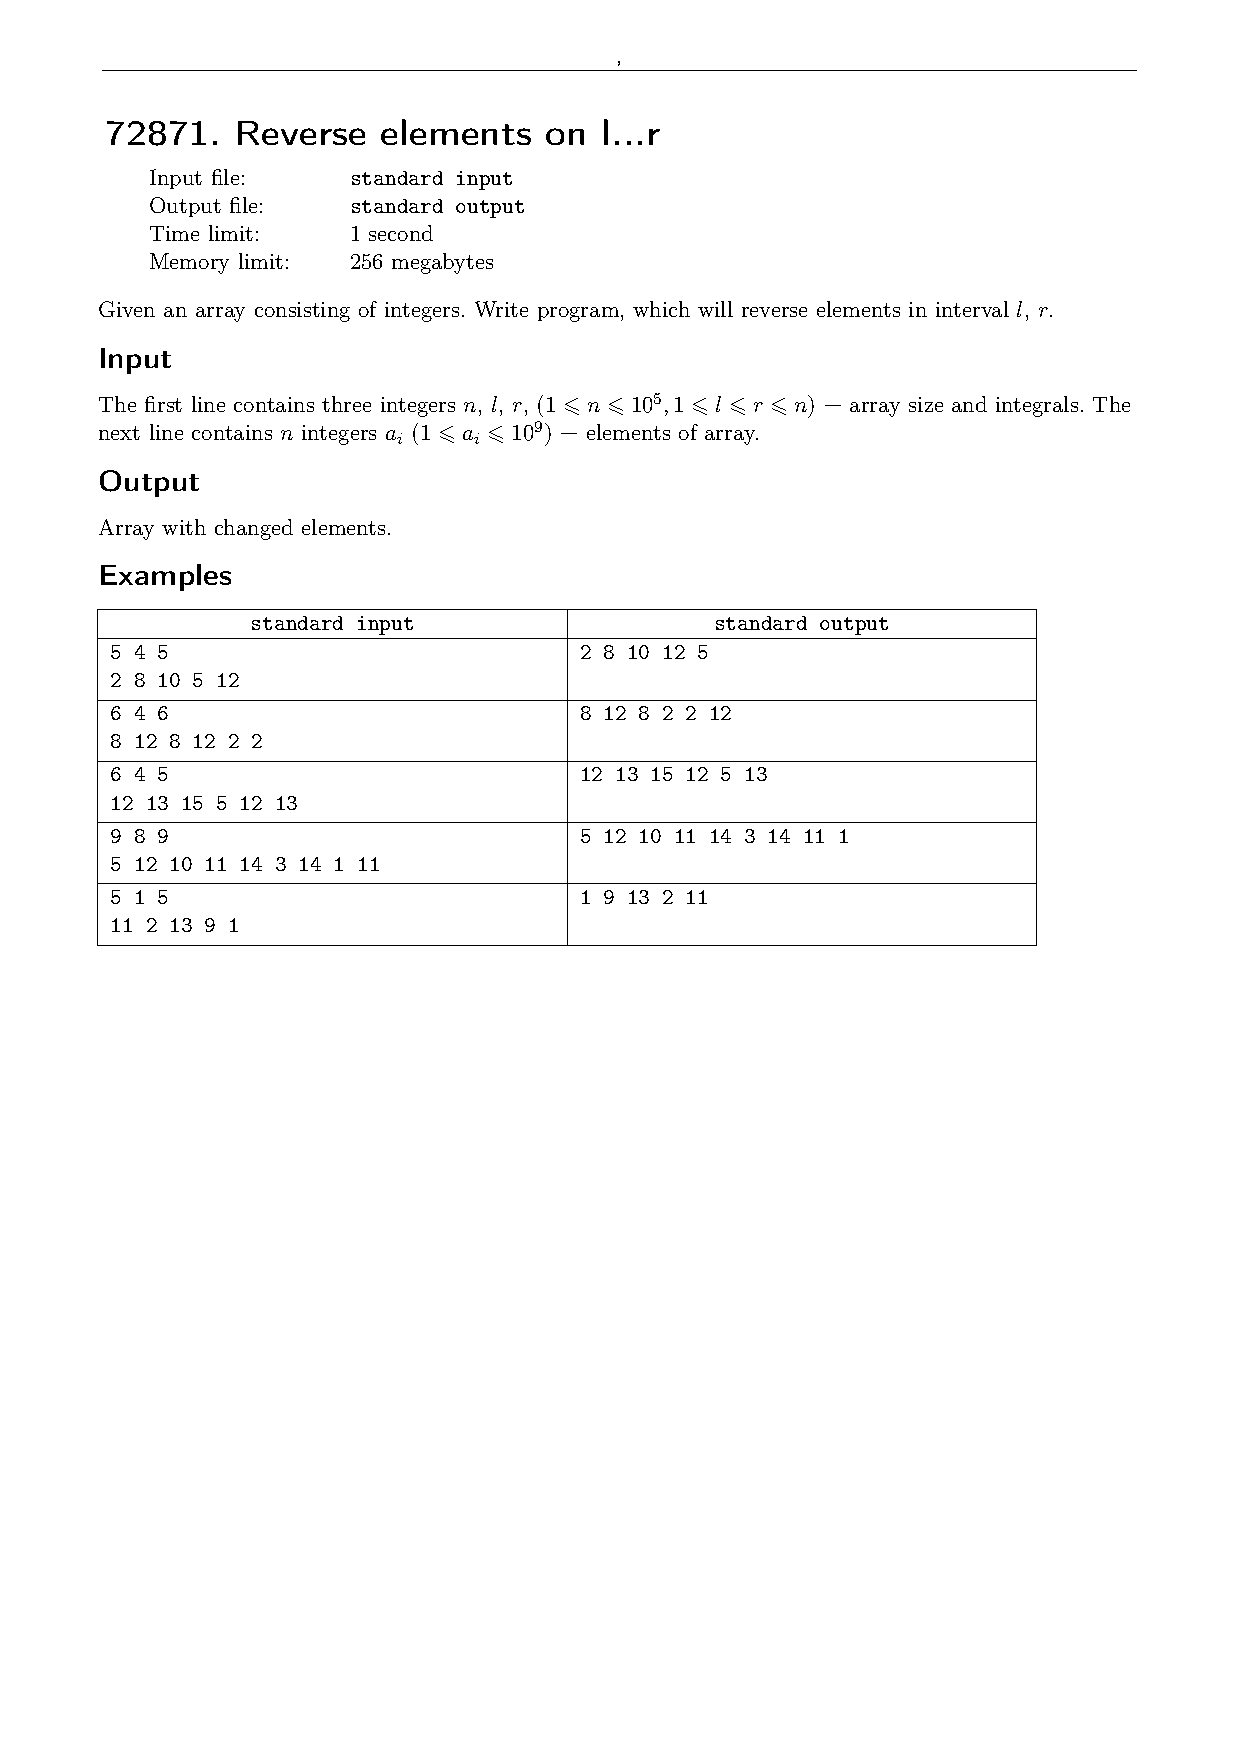
\includepdf[pages=-]{72871.pdf}
        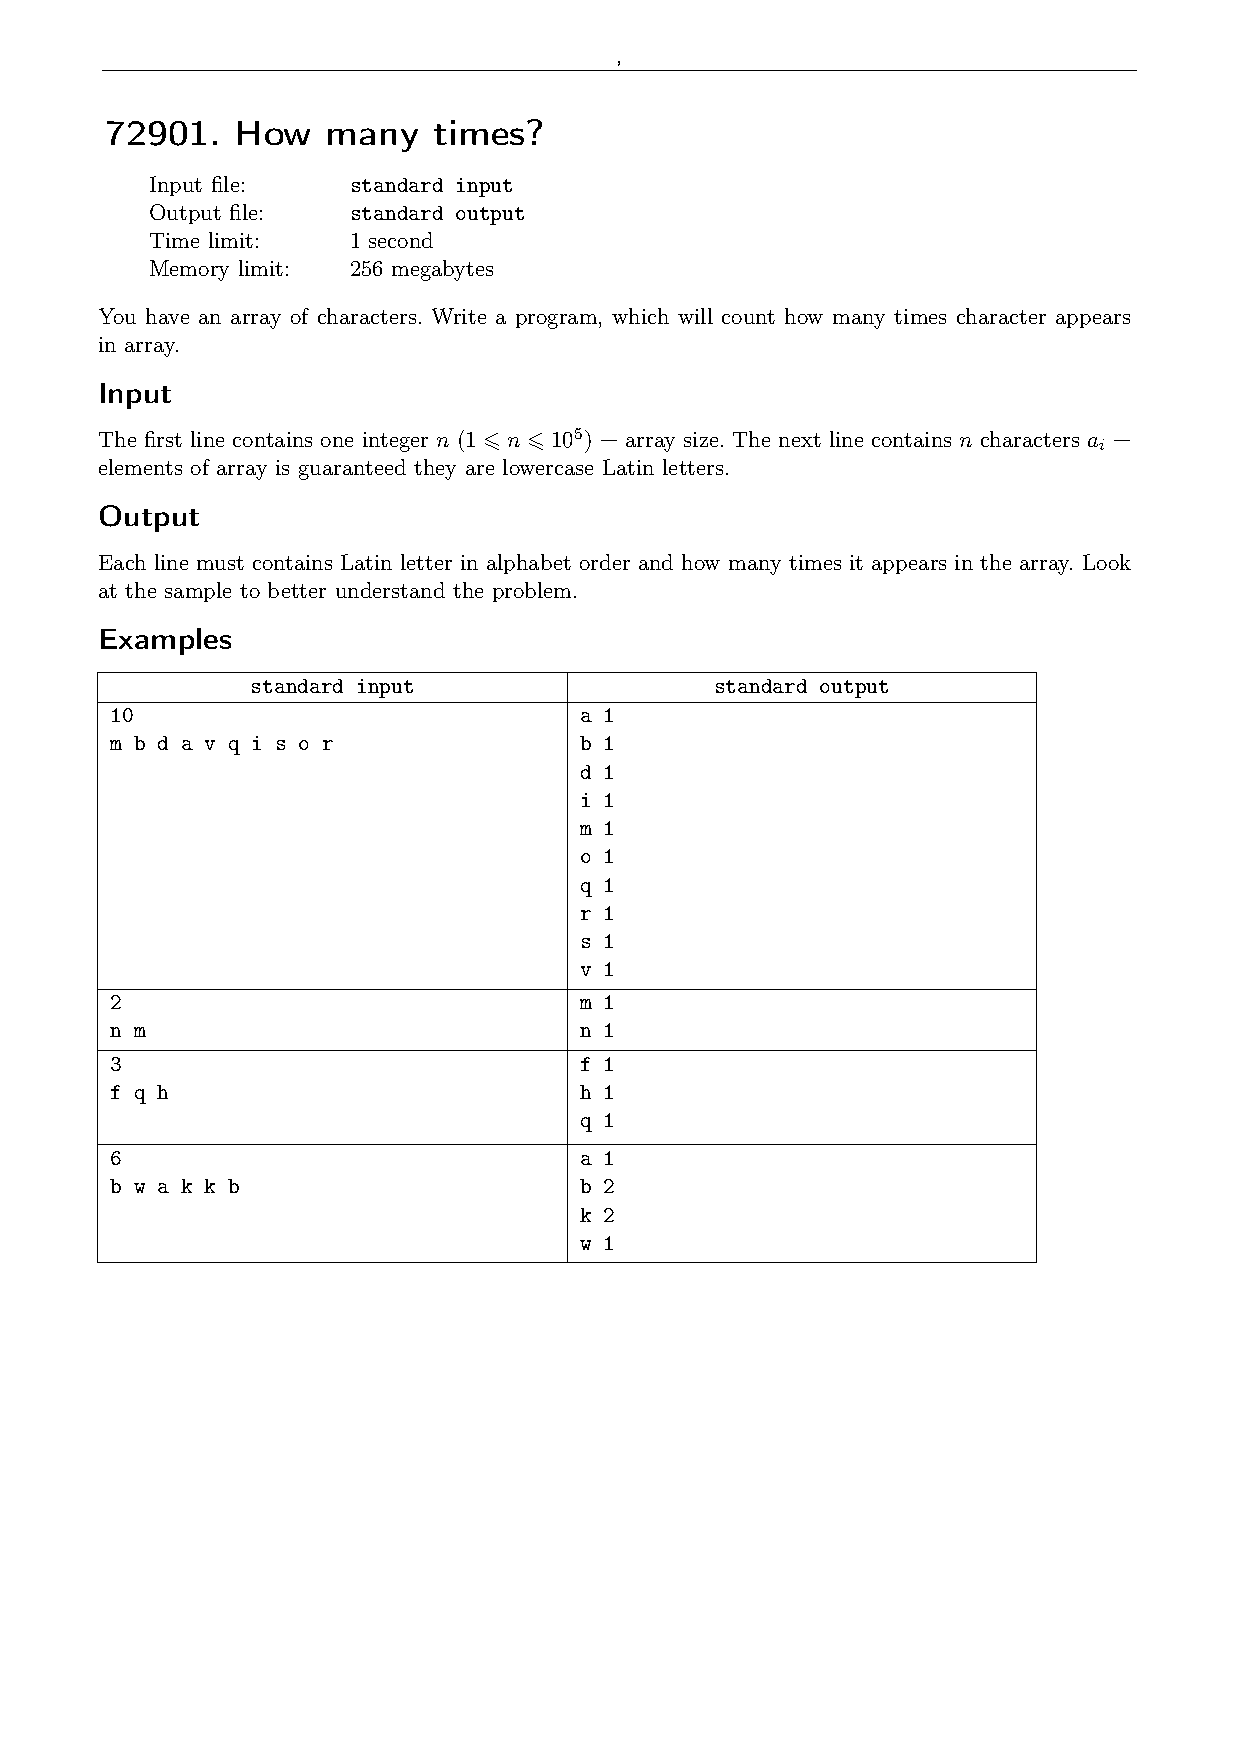
\includepdf[pages=-]{72901.pdf}
        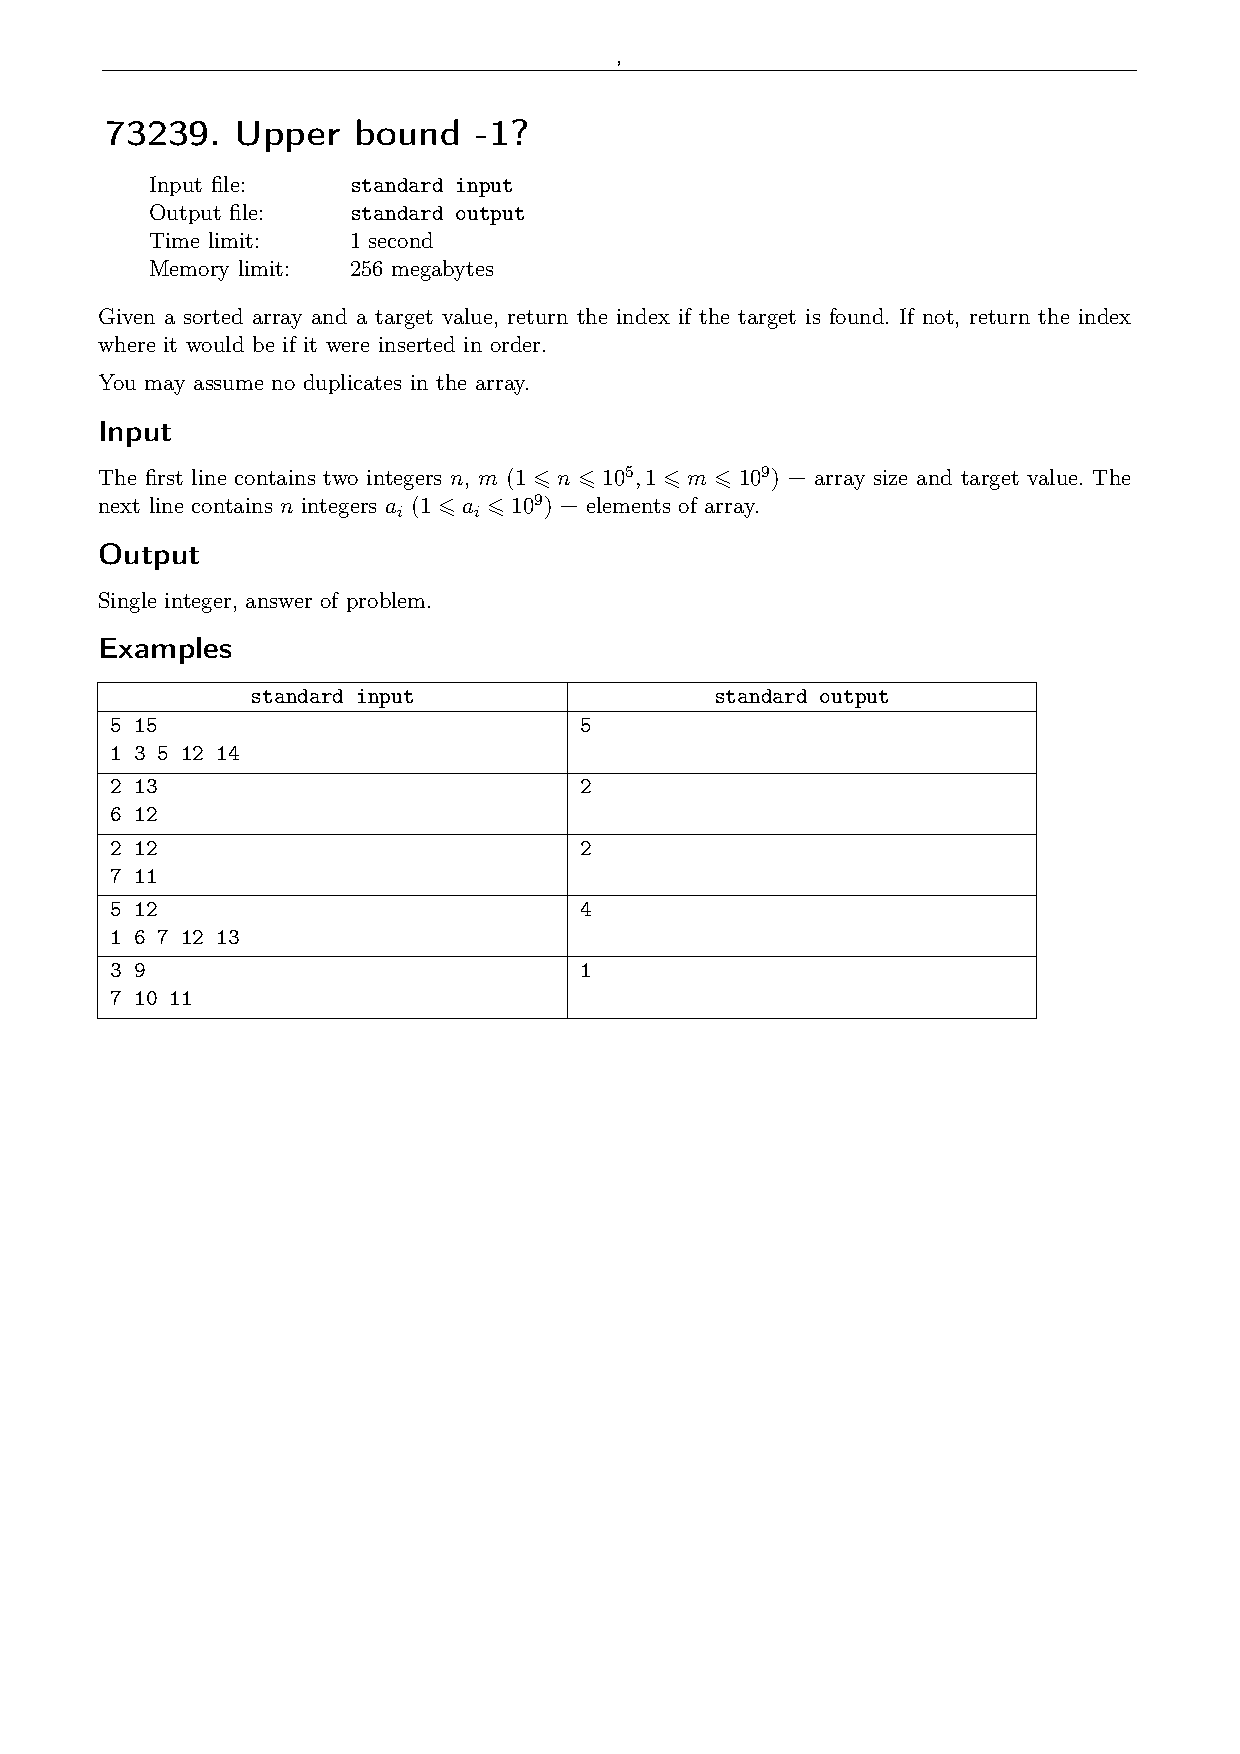
\includepdf[pages=-]{73239.pdf}
        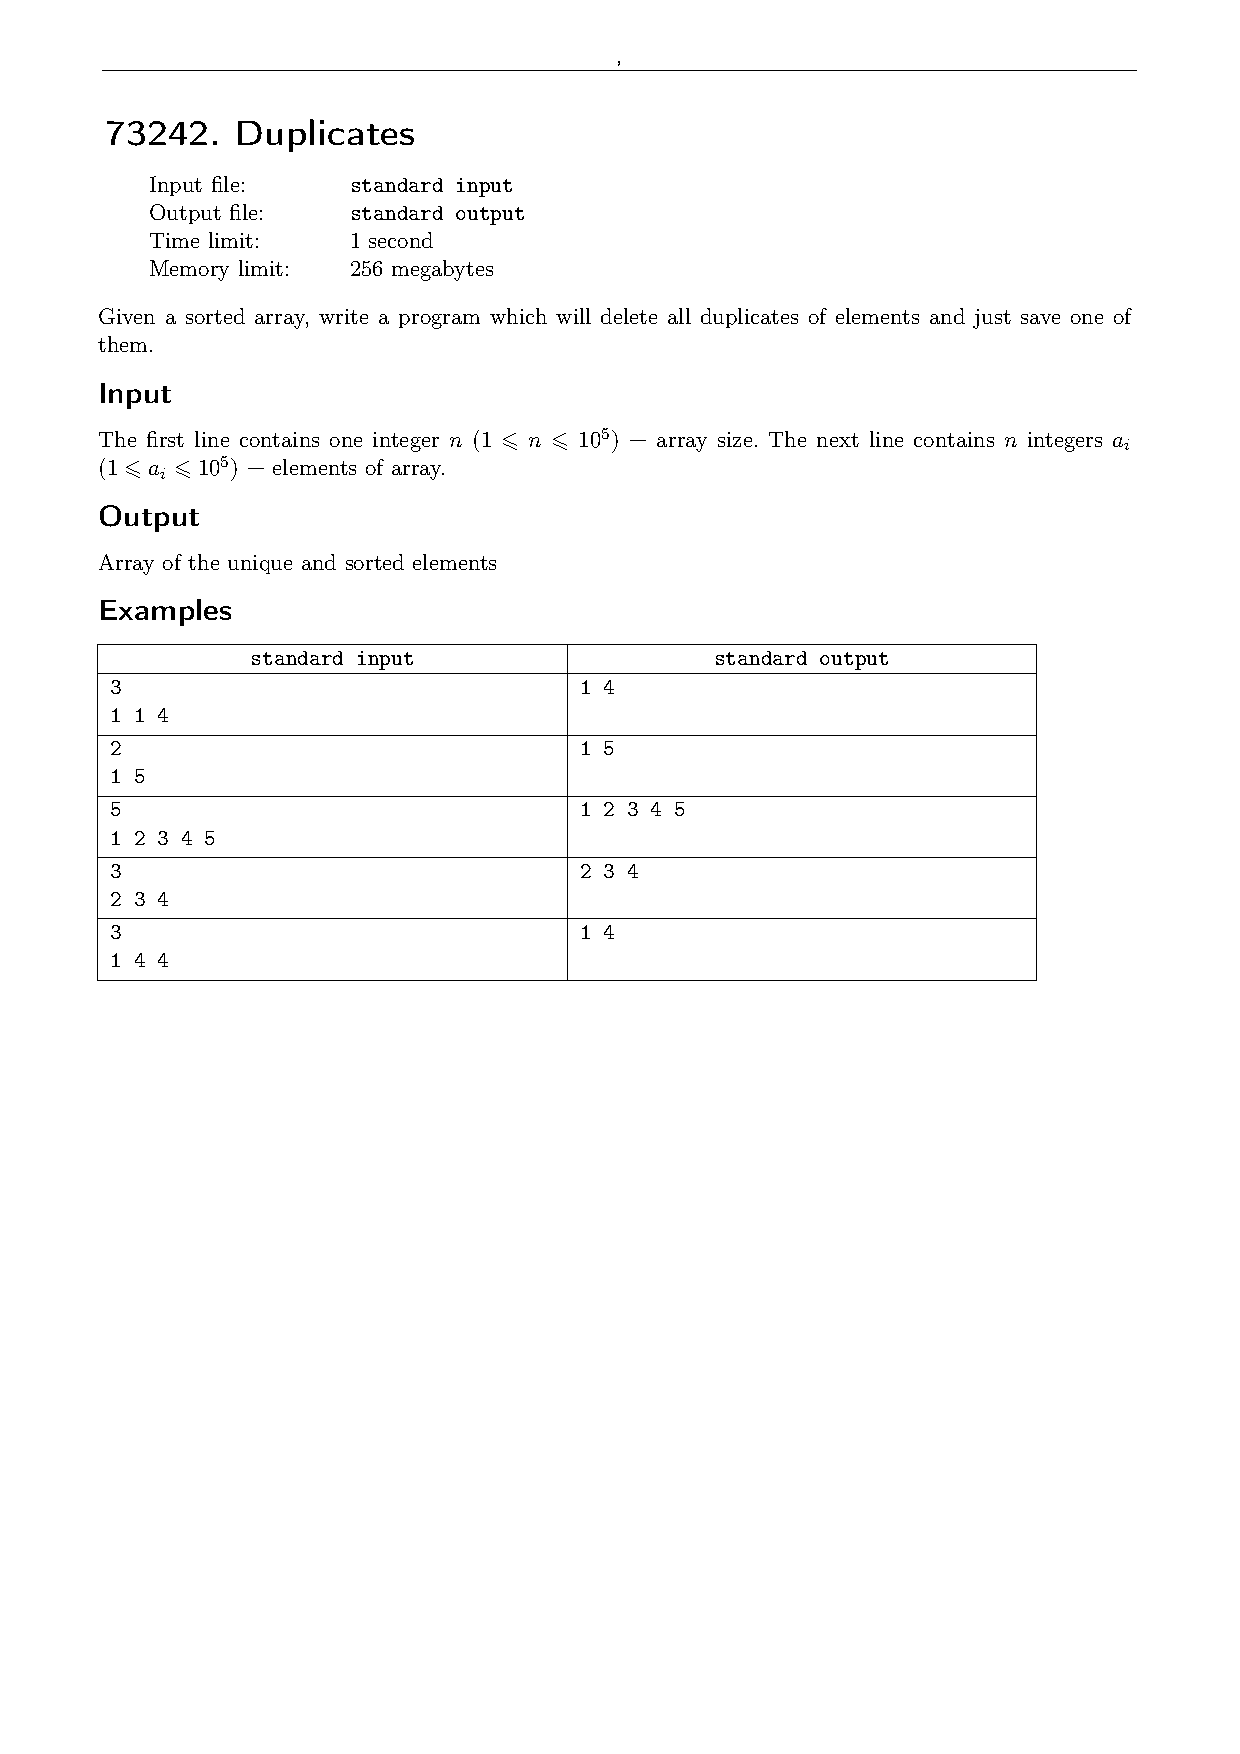
\includepdf[pages=-]{73242.pdf}
        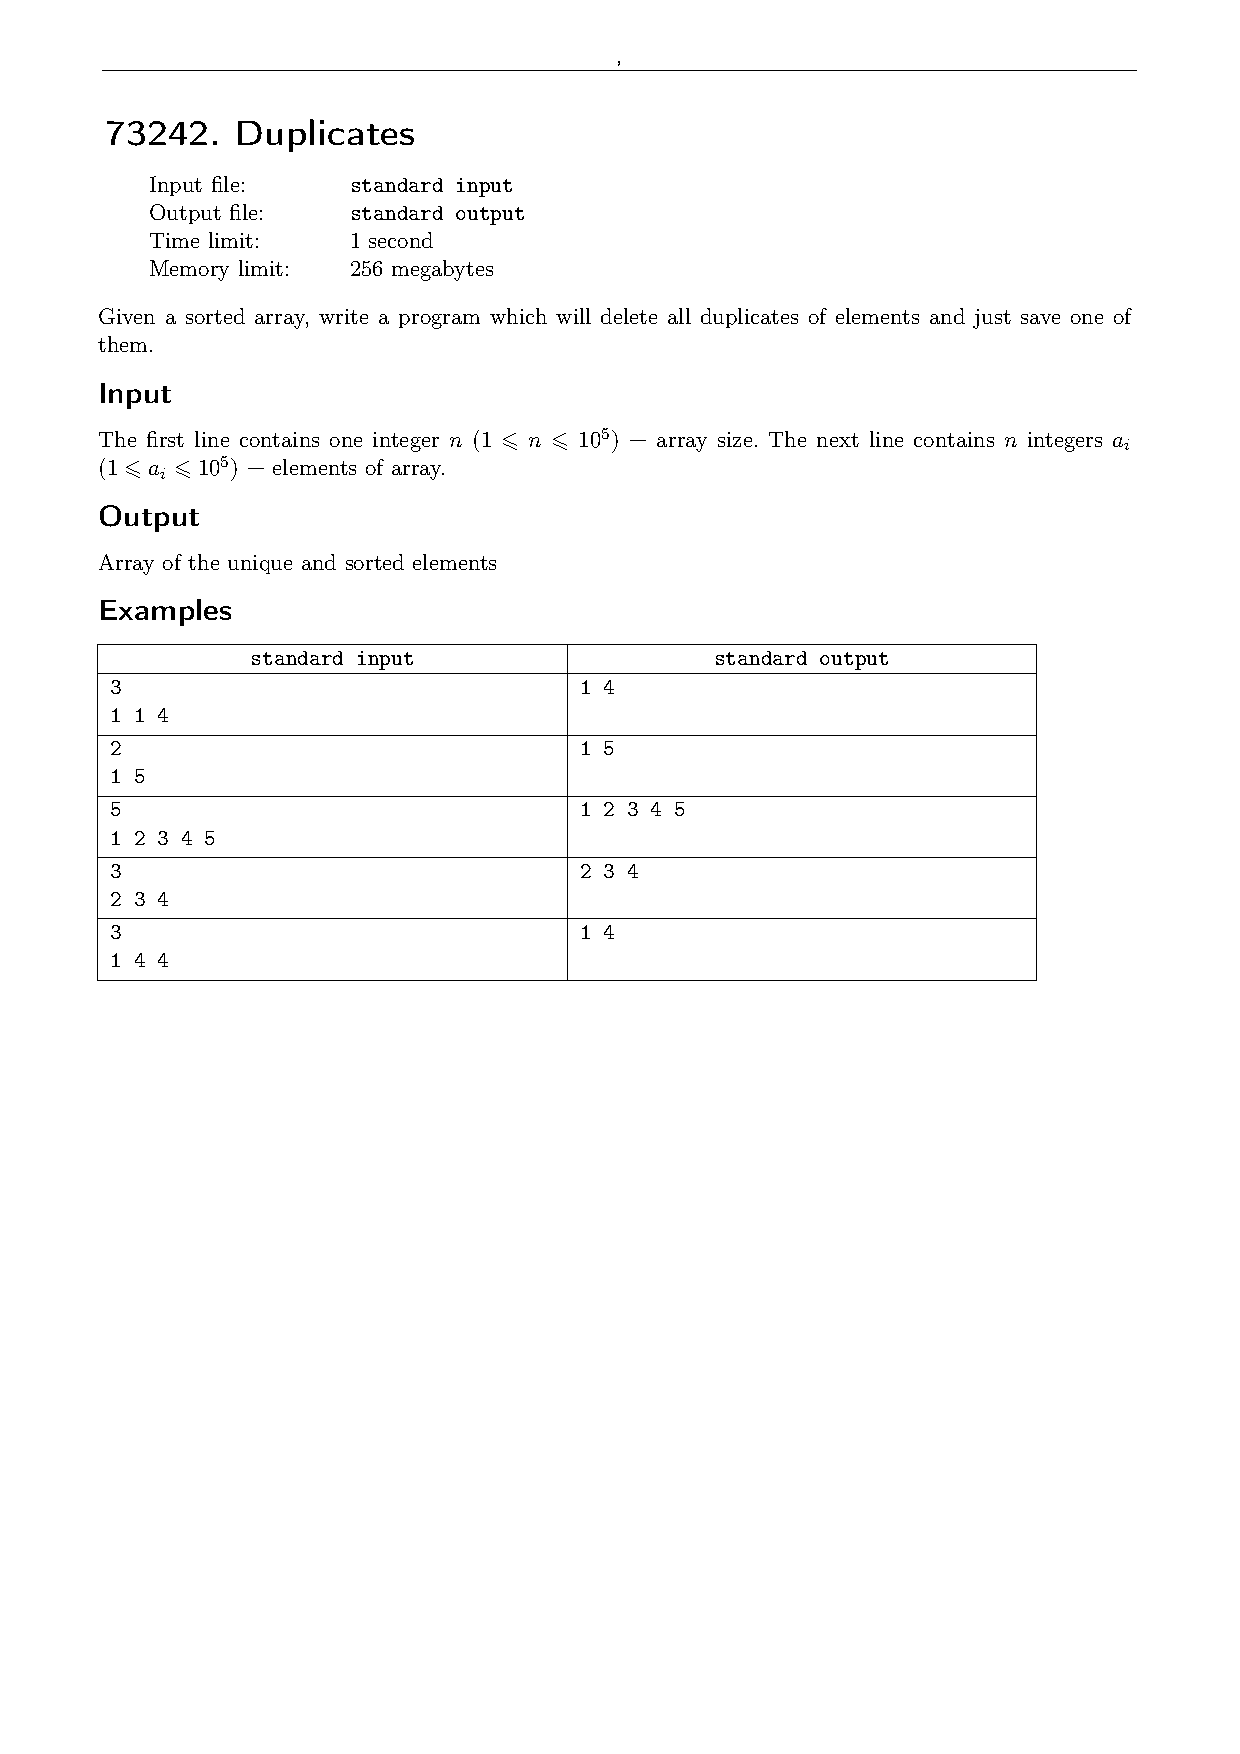
\includepdf[pages=-]{73242.pdf}
        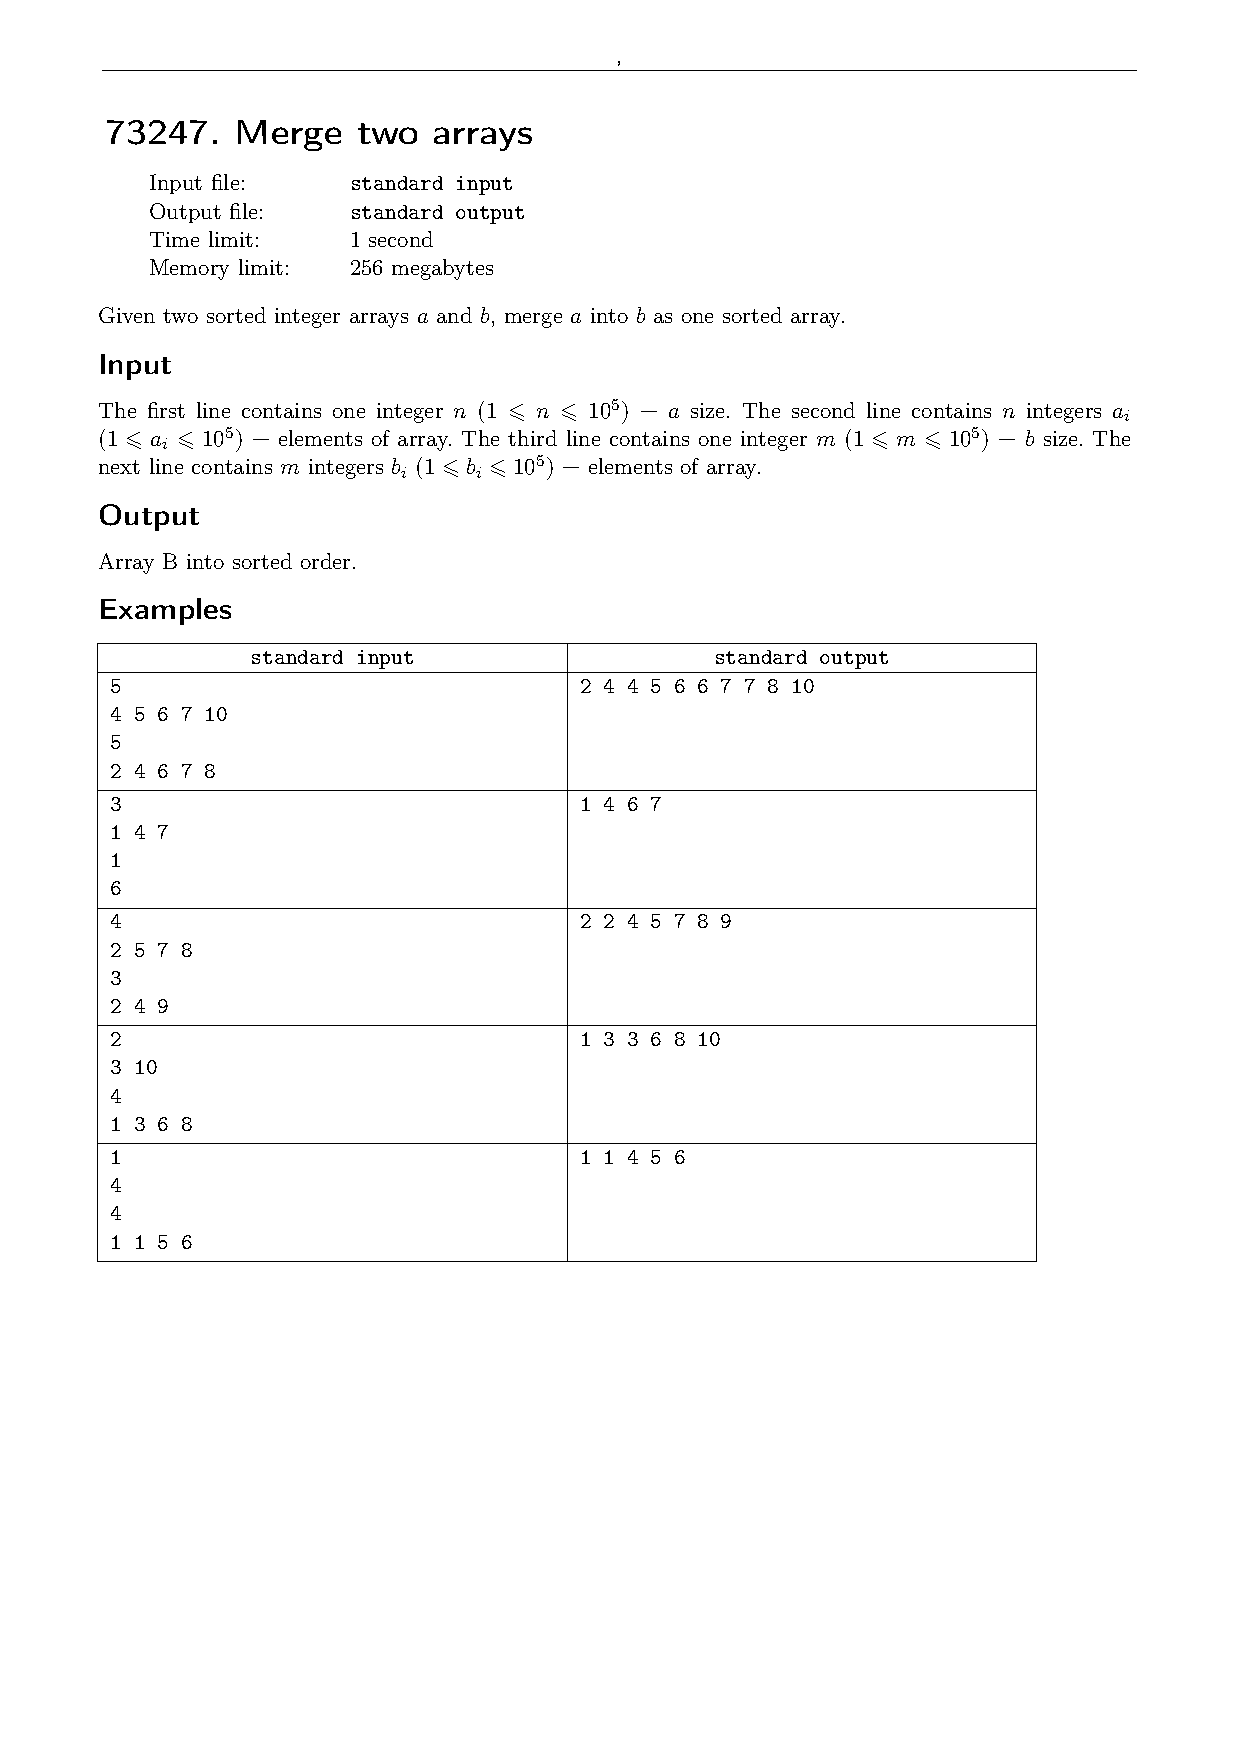
\includepdf[pages=-]{73247.pdf}
        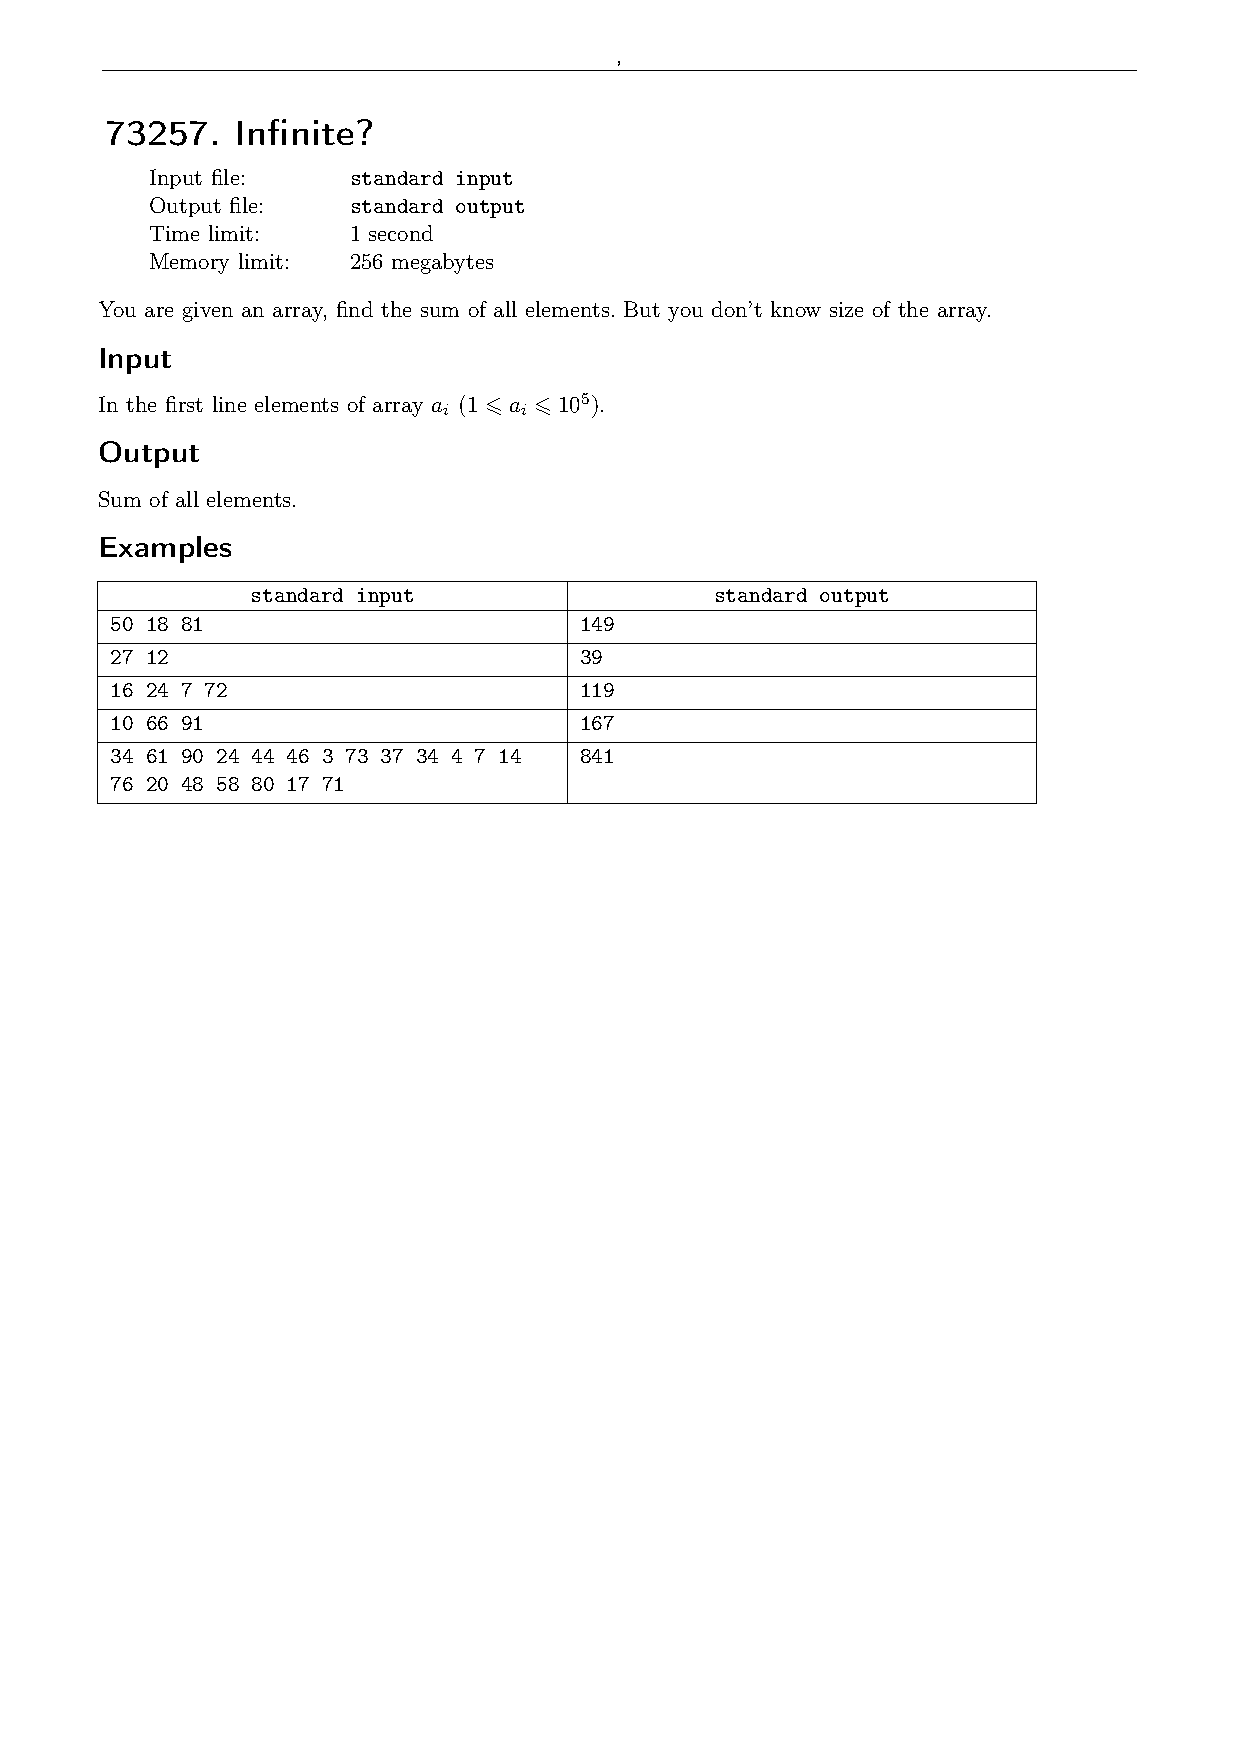
\includepdf[pages=-]{73257.pdf}
        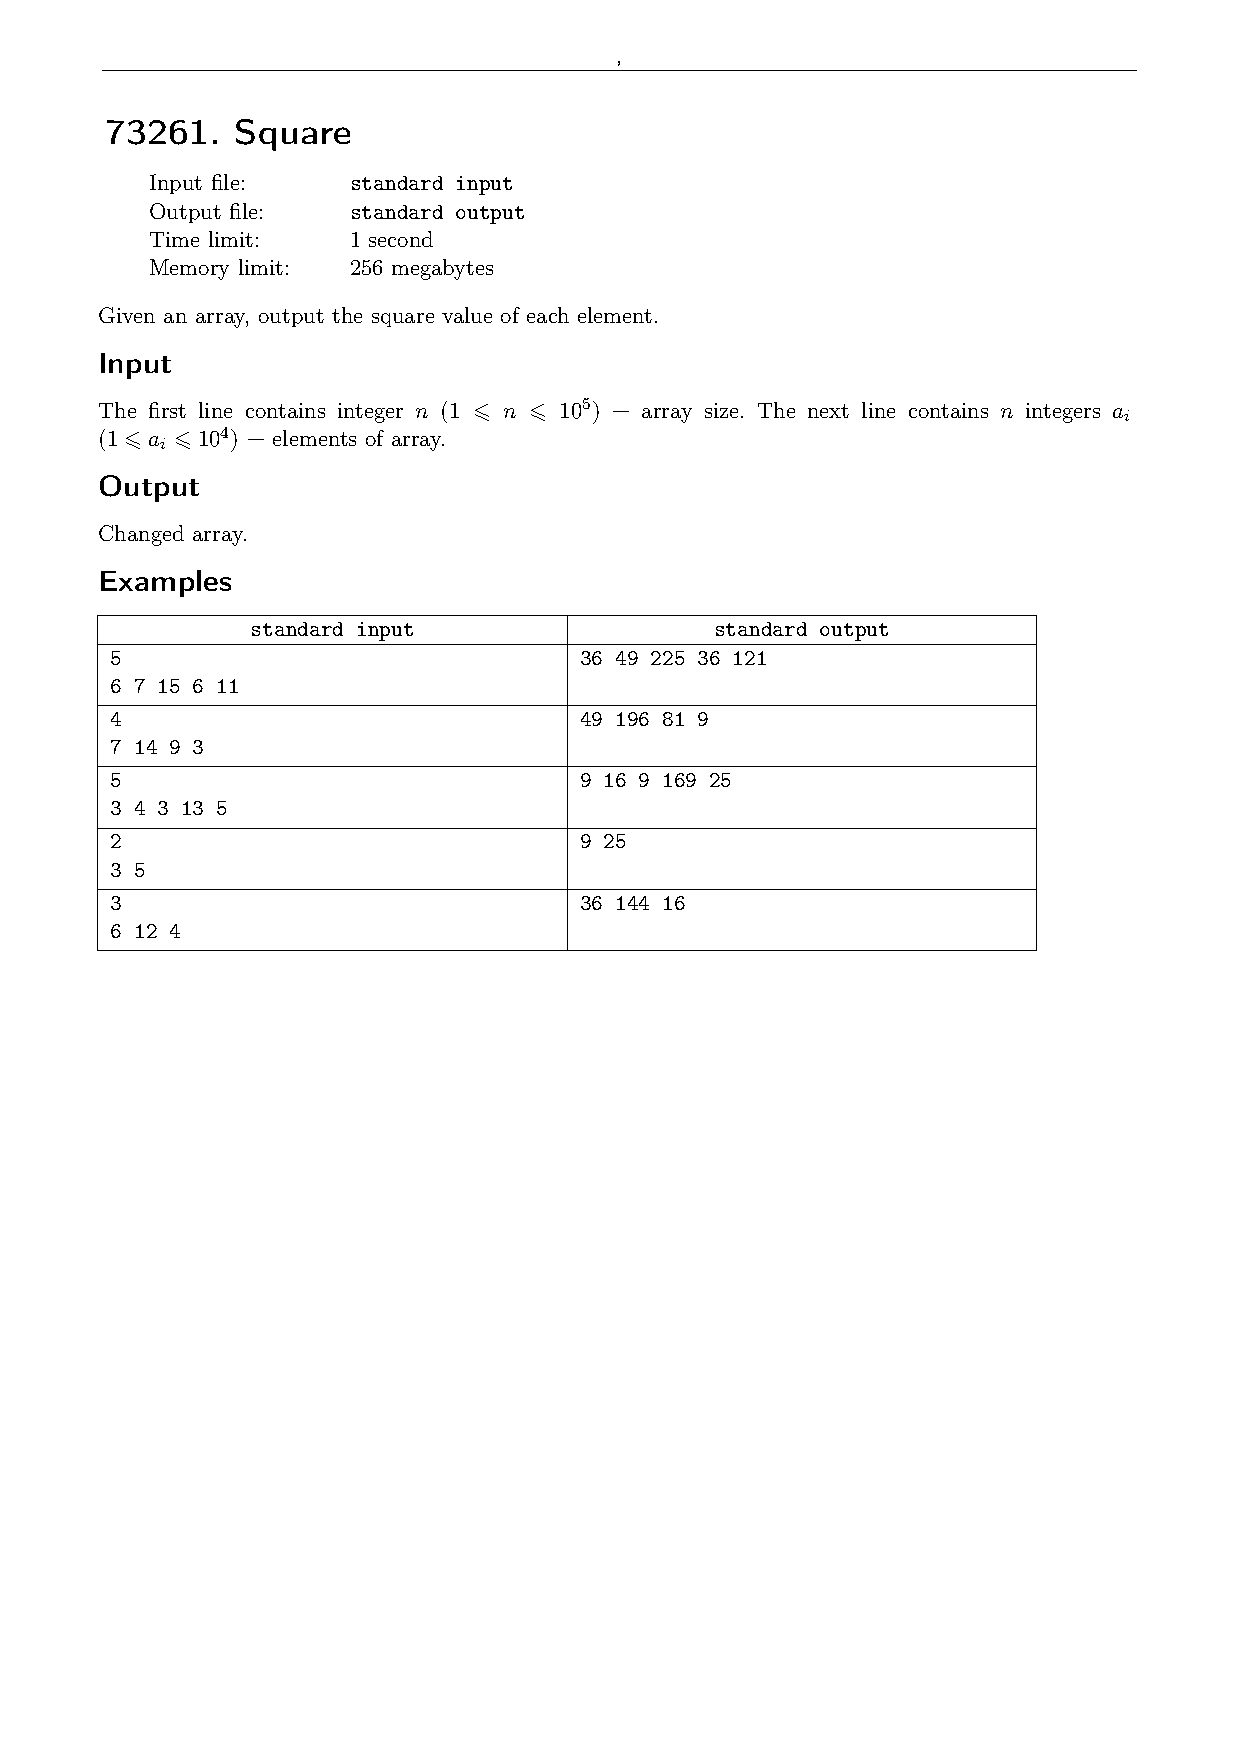
\includepdf[pages=-]{73261.pdf}
        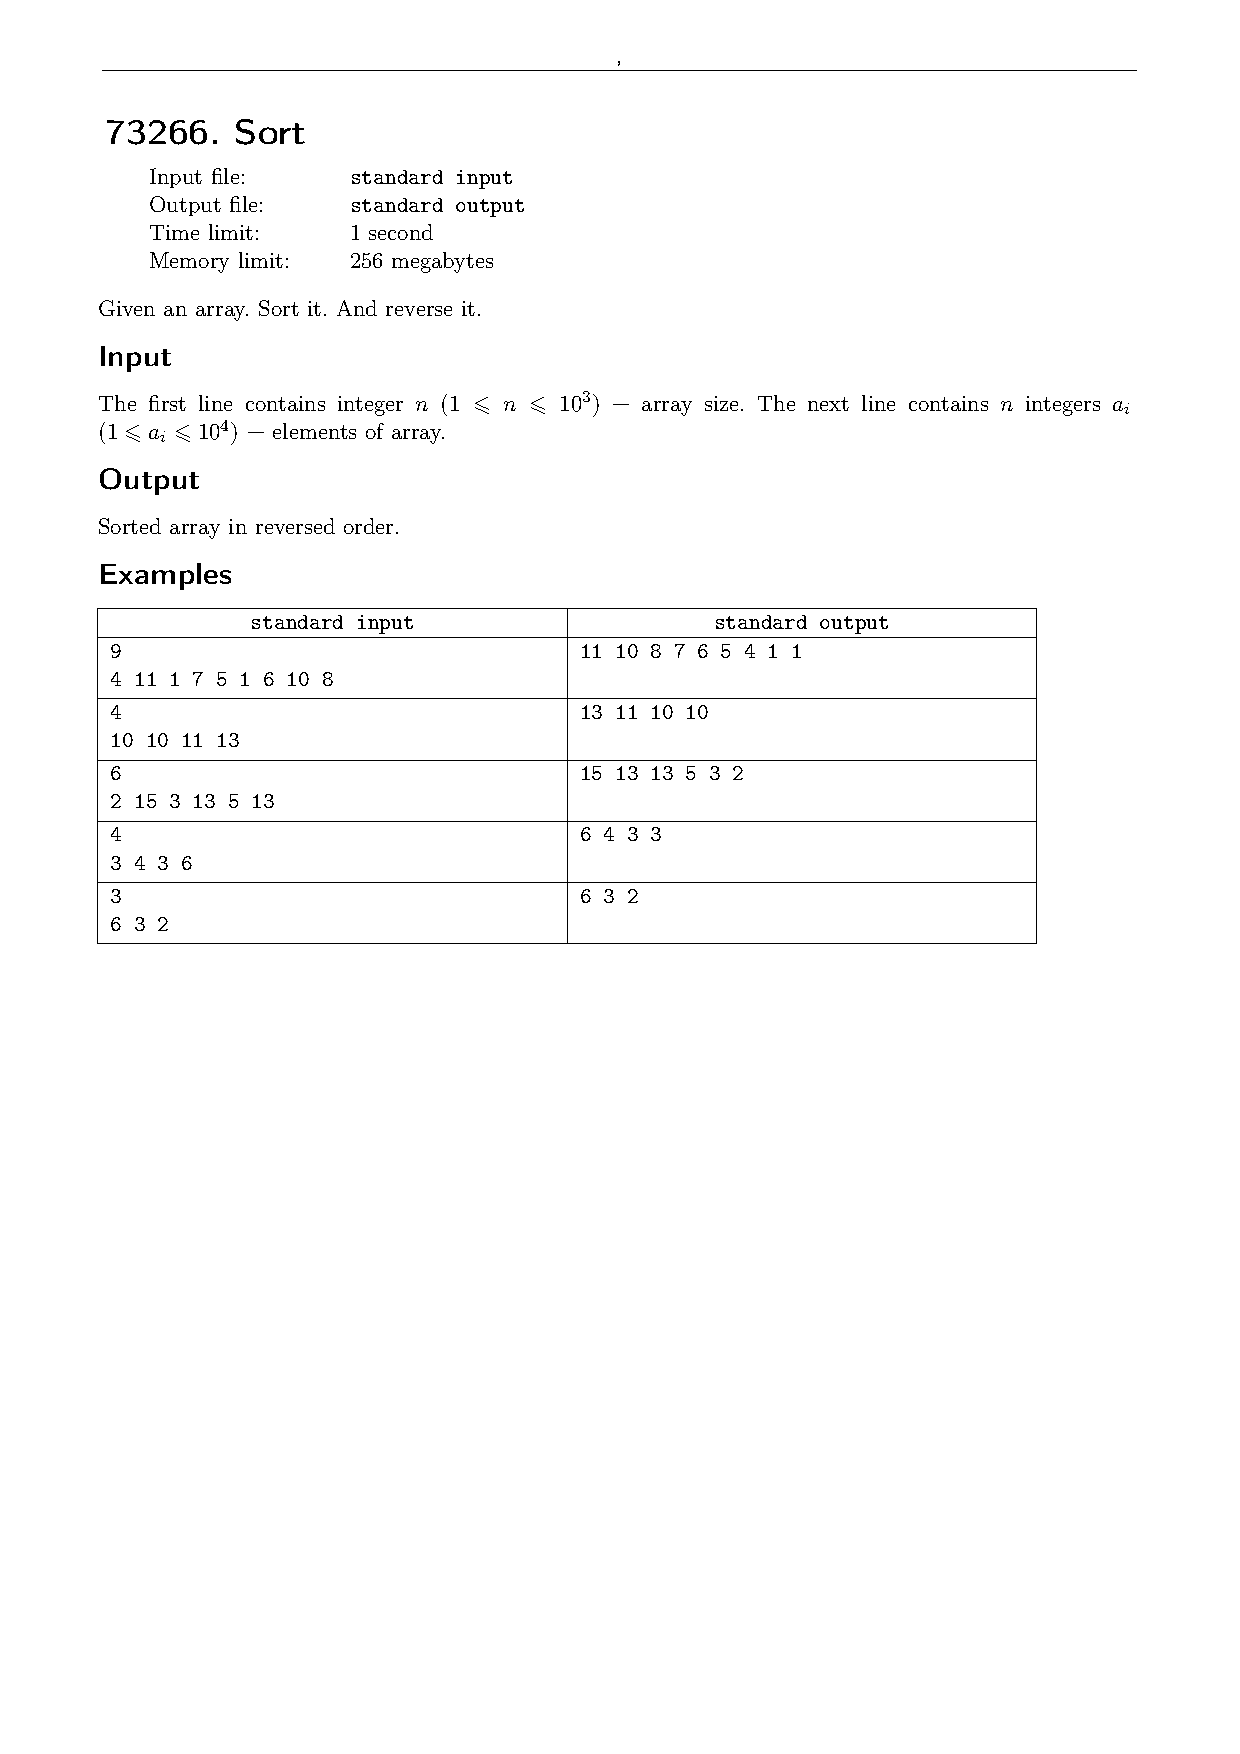
\includepdf[pages=-]{73266.pdf}
        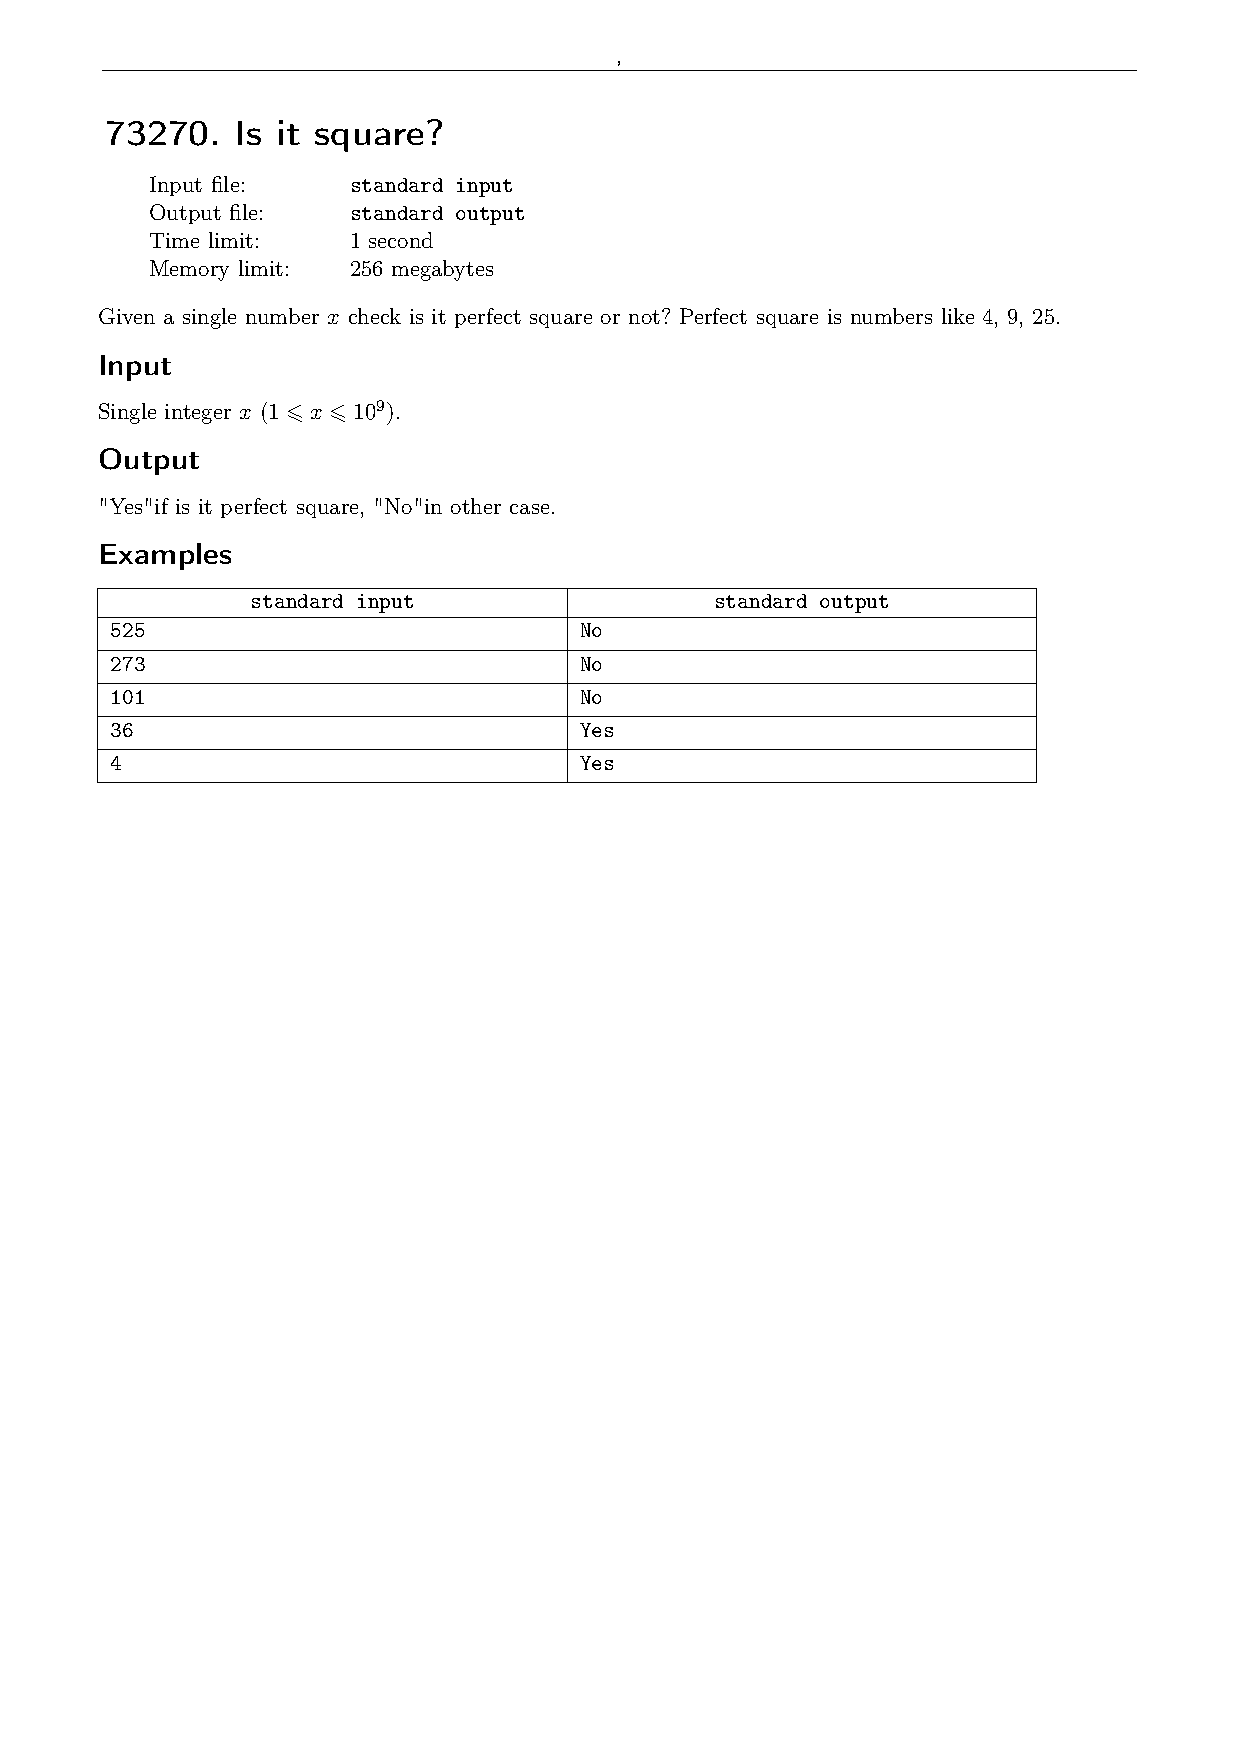
\includepdf[pages=-]{73270.pdf}
        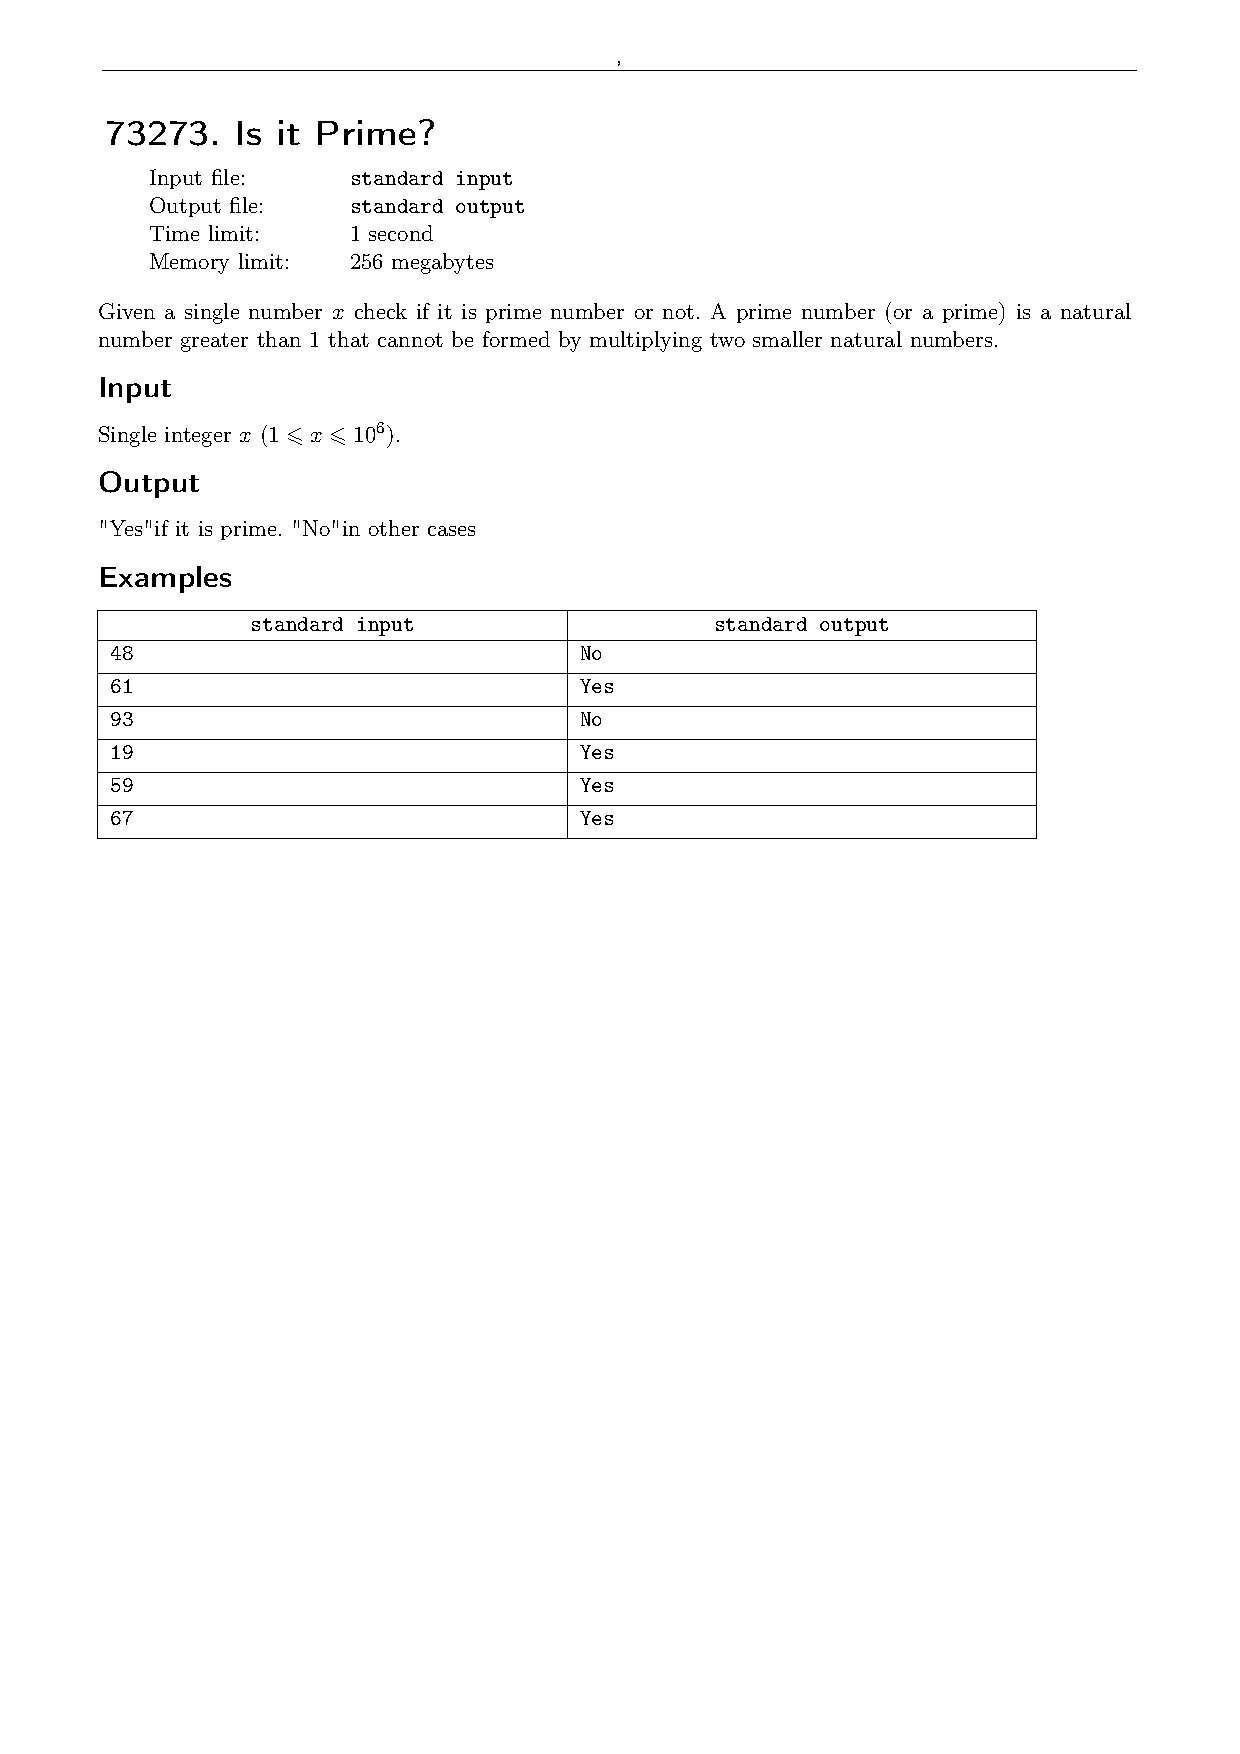
\includepdf[pages=-]{73273.pdf}

    \section{Lab Contest}
        \small
        All given task are emplaced in automated checker system for \textbf{lab3}:
        \\ \url{http://acm.kbtu.kz/cgi-bin/new-register?action=211&contest_id=127}
        \\ Feel free to submit your solutions without attempt count penalty.
        
    \section{Solutions}
        \textbf{Problem 72477}
        \lstinputlisting{72477.cpp}
        \textbf{Problem 72485}
        \lstinputlisting{72485.cpp}
        \textbf{Problem 72568}
        \lstinputlisting{72568.cpp}
        \textbf{Problem 72569}
        \lstinputlisting{72569.cpp}
        \textbf{Problem 72763}
        \lstinputlisting{72763.cpp}
        \textbf{Problem 72764}
        \lstinputlisting{72764.cpp}
        \textbf{Problem 72768}
        \lstinputlisting{72768.cpp}
        \textbf{Problem 72780}
        \lstinputlisting{72780.cpp}
        \textbf{Problem 72783}
        \lstinputlisting{72783.cpp}
        \textbf{Problem 72871}
        \lstinputlisting{72871.cpp}
        \textbf{Problem 72901}
        \lstinputlisting{72901.cpp}
        \textbf{Problem 73239}
        \lstinputlisting{73239.cpp}
        \textbf{Problem 73242}
        \lstinputlisting{73242.cpp}
        \textbf{Problem 73247}
        \lstinputlisting{73247.cpp}
        \textbf{Problem 73257}
        \lstinputlisting{73257.cpp}
        \textbf{Problem 73261}
        \lstinputlisting{73261.cpp}
        \textbf{Problem 73266}
        \lstinputlisting{73266.cpp}
        \textbf{Problem 73270}
        \lstinputlisting{73270.cpp}
        \textbf{Problem 73273}
        \lstinputlisting{73273.cpp}


    \section{Additional tasks for this lab}
    You can solve problems starting from A to J from the link below:\\
    \url{https://informatics.msk.ru/mod/statements/view.php?id=208}\\
    \textit{note: statements are in russian}

\end{document}